\chapter{Introdução}\label{Cap:Introduction}

% \section{Motivation}

Streaming de vídeo esféricos, ou vídeos 360°, é uma relativamente nova aplicação multimídia para realiadade virtual (do inglês VR - Virtual Reality) que chamou muita atenção nos últimos anos com a população dos óculos de realidade virtual, também conhecidos como visor de cabeça (do inglês HMD - Head Mounted Display) e o lançamento do Metaverso pela Meta. Como apresentado na figura~\ref{fig:video360}, os vídeos esféricos (ou vídeo 360°) são projetados e reproduzidos na casca interna de uma esfera e o usuário é posto no centro. Usando informações dos sensores de movimento do HMD, o usuário tem liberdade para olhar ao redor movendo a cabeça em três graus de liberdade enquanto o HMD exibe o vídeo em uma janela de visualização chamada viewport. Além dos HMD os vídeos esféricos também podem ser reproduzidos em dispositivos celulares, aplicativos desktop e navegadores web através do movimento do mouse. Esta facilidade permite que praticamente qualquer dispositivo reproduza os vídeos esféricos facilitando seu acesso.

\begin{figure}[h]
	\centering
	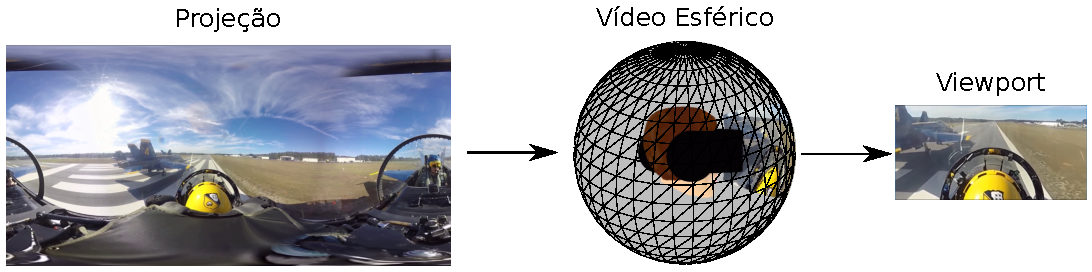
\includegraphics[width=0.8\columnwidth]{fig/viewport.pdf}
	\caption{Em um vídeo esférico uma projeção é usada como textura de uma esfera 3D com o usuário no centro que poderá mover a cabeça e olhar ao redor usando seu HMD.}
	\label{fig:video360}
\end{figure}

De todas as aplicações para VR, o streaming de vídeo esférico é o que possui a maior taxa de bits, pois toda a projeção é transmitida em Ultra Alta Definição (do inglês UHD - Ultra High Definition). De acordo com~\cite{Zhou2017, Liu2017}, empresas como YouTube e Facebook usam a arquitetura tradicional de streaming de vídeo 2D para transmitir a projeção dos vídeos esféricos. Inicialmente a projeção é comprimida com H.264 ou VP9 e disponibilizados através do manifestos de protocolos com o Dynamic Adaptive Streaming over HTTP (DASH) que disponibilizam segmentos de vídeo com duração constante, codificados sob diversas qualidades/taxas de bits diferentes. Assim, analisando o buffer e/ou a largura de banda disponível, a aplicação cliente poderá mudar a qualidade da reprodução de acordo com a disponibilidade dos recursos do dispositivo. Por exemplo, o tocador do vídeo poderá reduzir a qualidade se a largura de banda disponível for reduzida ou se a bateria estiver acabando.

No entanto, ao contrário dos vídeos 2D, um usuário deve visualizar apenas uma fração de todo o vídeo esférico devido à limitação do campo de visão humano (FOV). Conforme mostrado na Figura~\ref{fig:viewport1}(a), a região do vídeo que é exibido no HMD é chamada viewport e todos os pixels fora desta região não serão visualizados pelo usuário. Dependendo do fabricante do HMD o FOV pode variar, mas geralmente possui $\times90^{\circ}$ de abertura vertical e de $120^{\circ}$ a $90^{\circ}$ de abertura horizontal, o que corresponde a aproximadamente 16\% da esfera~\cite{Afzal2017}. Por isso, para garantir boa qualidade exibida no HMD, a projeção deve ser codificada em alta resolução, resultando em arquivos muito grande e necessitando de tanta largura de banda quanto for a qualidade da codificação. 

\begin{figure}[h]
        \centering
        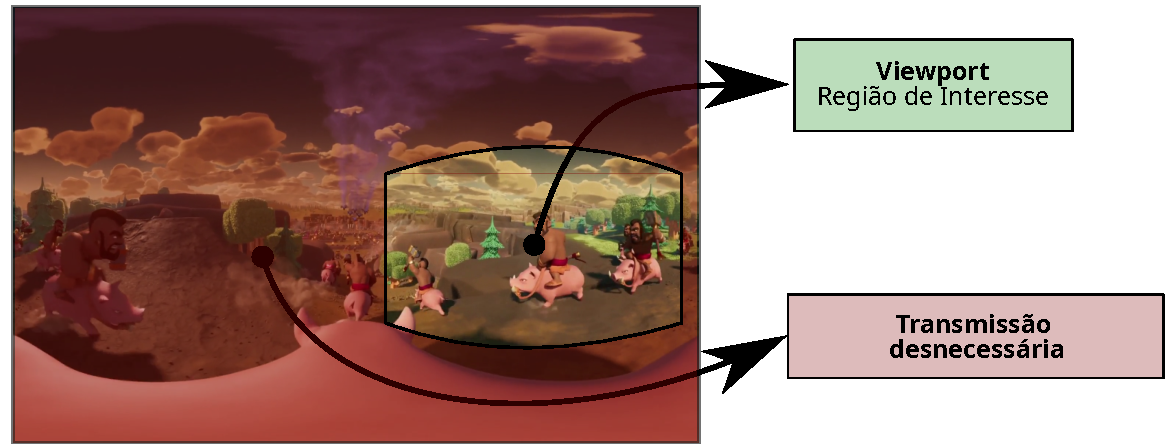
\includegraphics[width=0.80\columnwidth]{fig/viewport1.pdf}
        \caption{Viewport em um streaming com ladrilhos: desperdício ao requisitar pixels não vistos (em vermelho).}
        \label{fig:viewport1}
\end{figure}

Desta forma, transmitir toda a projeção pode desperdiçar diversos recursos do sistema como largura de banda, tempo de processamento, bateria, etc. Dispositivos móveis tendem a sofrer mais com este tipo de aplicação que podem ter sua bateria drenada rapidamente e sofrer aquecimento, enquanto que a conexão móvel é limitada e mais cara. Além disso, os algoritmos de Adaptação da Taxa de Bits (do inglês ABR - Adaptive Bitrate) usados pelo protocolo DASH utilizam informações sobre estes recursos para determinar a qualidade do vídeo que deve ser solicitada ao servidor. Caso não haja recursos suficientes o algoritmo reduz a qualidade do vídeo para conseguir manter a reprodução do vídeo constante.

Afim de economizar recursos, vários trabalhos~\cite{Alface2012, Zare2016, Qian2018, Liu2017, Graf2017, Xiao2018, Nasrabadi2019} sugerem uma abordagem baseada na segmentação espacial da projeção em vídeos independentes chamados ladrilhos, de modo que o cliente possa solicitar somente os ladrilhos em uma região de interesse (do inglês ROI - Region Of Interest) que serão vistos pelo usuário nos próximos segundos. A figura~\ref{fig:viewport2} apresenta esta abordagem utilizando um padrão de ladrilhamento $4 \times 4$. A ROI será todos os pixels cobertos pelos ladrilhos que tocam o viewport. Desta forma, somente os ladrilhos tocados pelo viewport poderão ser requisitados com maior qualidade, enquanto os ladrilhos não vistos serão transmitidos em baixa qualidade ou mesmo não serão transmitidos. 

\begin{figure}[h]
	\centering
	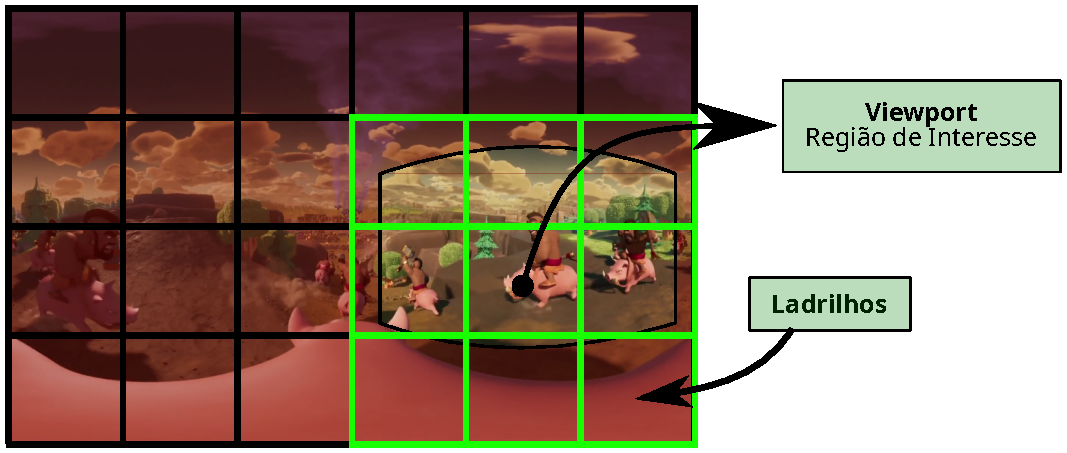
\includegraphics[width=0.80\columnwidth]{fig/viewport2.pdf}
	\caption{Um vídeo ladrilhado no formato $6 \times 4$ com região de interesse em verde. Apenas essa região é necessária para o viewport do usuário.}
	\label{fig:viewport2}
\end{figure}

Porém, a partir desta abordagem surgem vários novos desafios. Como os chunks do protocolo DASH possuem duração fixa de vários segundos e o usuário pode mover o viewport para fora do grupo de ladrilhos inicialmente apresentados, é necessário prever o movimento do usuário durante toda a duração do chunk. Uma predição de viewport errada solicitará um conjunto de chunks errados exigindo uma nova requisição dos ladrilhos faltantes, desperdiçando largura de banda e em alguns casos o vídeo poderá travar até que o chunk correto chegue, seja decodificado e desenhado na tela. O algoritmo ABR passa a ter que lidar com os erros de predição de viewport e restrições como por exemplo, não misturar ladrilhos de qualidades diferentes no viewport e a classificação das requisições dos ladrilhos em níveis de prioridade. Além disso, podemos observar que quanto maior a segmentação (e menor os ladrilhos), menos pixels ficarão fora do viewport. Porém, quanto menor o ladrilho, menor o espaço de busca do compensador de movimento dos codificadores, reduzindo a eficiência da compressão e, por fim, aumentando a taxa de bits. Outro problema que surge é que a segmentação da projeção em ladrilhos independentes exigirá que o cliente utilize várias instâncias do decodificador trabalhando em paralelo. Desta forma, quanto maior o ladrilhamento, mais decodificadores serão necessários instanciar e mais tempo de processamento será utilizado. Esta condição se torna crítica em dispositivos móveis que possuem menos poder computacional, onde o uso massivo de processamento poderá drenar a bateria muito rápido além de causar aquecimento.

Diversas propostas foram feitas afim de lidar com a predição de viewport e a seleção de chunks, porém é muito difícil realizar a comparação do desempenho de cada abordagem devido a natureza interativa da comunicação cliente-servidor. Submeter grupos de degradações a diferentes usuários afim de avaliar a qualidade subjetiva é a abordagem  recomendada pelo ITU-T afim de avaliar a qualidade subjetiva do vídeo esférico~\cite{ITU-ITU-TRecommendationP.9192020}. Porém, é muito difícil controlar o que o usuário verá, pois a cada reprodução do vídeo esférico com ladrilhos, os usuários terão um comportamento completamente diferente. Inclusive, se um vídeo for assistido por um mesmo usuário várias vezes, seu comportamento será diferente a cada reprodução. Cada ladrilho que foi codificado individualmente com a mesma qualidade visual possuirá diferentes taxas de bits dependendo do seu conteúdo e cada usuário solicitará um diferente conjunto de ladrilhos ao servidor dependendo de onde estará olhando e da velocidade de movimento da cabeça, que por sua vez requererá diferentes recursos do computador e terá diferentes qualidades de experiência (do inglês QoE - Quality of Experience).

Afim de permitir a reprodutibilidade do comportamento do usuário sob diferentes algoritmos ABR e preditores de movimento de cabeça, este trabalho propõe um fluxo de trabalho e construção de um banco de dados com diversas métricas objetivas que poderão ser usadas para emular um sistema de transmissão de vídeo e replicar o comportamento dos usuários. A velocidade angular do movimento de cabeça é uma das características que mais afetam o preditor de viewport~\cite{Qian2016}, porém, de acordo com o estudo de~\cite{Nasrabadi2019}, usuários que movimentam muito em vídeos de uma categoria arbitrária, tendem a se movimentar muito também em todas as outras categorias. Desta forma, podemos supor de forma cuidadosa que o usuário teria um comportamento aproximadamente semelhantes se houvesse pequenas variações de qualidade e assim extrair uma representação aproximada da qualidade objetiva percebida sob as mais diversas restrições de sistema, que vão desde capacidade de processamento a variação da largura de banda disponível. Usando ferramentas de simulação de redes como NS-3, NS-2 ou OpNet ainda será possível modelar toda a arquitetura do sistema de transmissão, desde atrasos de rede controlados a consumo energético sob diferentes infraestruturas de comunicações, como 5G, Wi-Fi, satélite, redes ópticas, Ethernet, etc.

Até o momento não existe na literatura nenhum banco de dados que apresente os dados do streaming de vídeos processados da forma como propomos, onde a codificação é feita baseada na qualidade e não na taxa de bits usando o codificador HEVC. Optamos fazer a compressão usando o parâmetro CRF pois se a codificação for feita considerando a taxa de bits poderá haver grande desperdício de largura de banda com ladrilhos que são poucos complexos de codificar, como por exemplo o chão ou o teto. Além disso, caso os ladrilhos possuam grande diferença de qualidade dentro de uma mesma representação, haverá bordas em torno dos ladrilhos, o que degradará a qualidade de experiência.

O principal objetivo deste trabalho é criar um ambiente padronizado e controlado para a comparação de diferentes sistema de transmissão de vídeos esféricos segmentados em ladrilhos usando protocolos adaptativos como o DASH. No caminho, nossos objetivos específicos são: 

\begin{enumerate}
	\item Caracterizar os ladrilhos dos vídeos de diferentes categorias, sob diferentes projeções e segmentados em diferentes padrões de ladrilhamento. Extraímos a taxa de bits, medimos o tempo de decodificação para cada chunk e calculamos diversas métricas de qualidade objetivas baseadas no erro quadrático médio tanto das projeções quanto do viewport exbido ao usuário.
	
	\item Estimar o limite inferior de recursos necessários para a reprodução dos vídeos esféricos para diferentes usuários. Usando o banco de dados de movimento de cabeças disponibilizado no trabalho de Nasrabadi~\cite{Nasrabadi2019}, extraímos o comportamento das requisições dos ladrilhos em um caso ideal e calculamos a qualidade do vídeo apresentado no viewport em termos do MSE. Aproveitando a taxonomia desenvolvida por Nasrabadi ainda agrupamos os resultados considerando o tipo de movimento da câmera e o numero de objetos em movimento no vídeo.
	
	\item Desenvolver um conjunto de ferramentas para manipulação das projeções equirretangular e cubemap, conversões de coordenadas 3D e 2D, extração do viewport, seleção de ladrilhos e cálculo de métricas de qualidade.
\end{enumerate}

O restante deste estudo está organizado da seguinte forma: No Capítulo 2, é realizada uma revisão do estado da arte para datasets de métricas de vídeo esférico segmentado em ladrilhos, considerando mecanismos de seleção de blocos, previsão de janela de visualização e bancos de dados disponíveis. O capítulo 3 concentra-se na modelagem do Sistema e métricas propostas. O capítulo 4 relata as análises de diferentes cenários e as características específicas deste dataset, por fim, no capítulo 5 são apresentadas as conclusões do trabalho desenvolvido e as propostas de trabalhos futuros para a continuação desta pesquisa.


 \chapter{Trabalhos relacionados}


%Nessa linha, Qian et al.~\cite{Qian2018} propuseram uma solução baseada em ladrilhos voltada para dispositivos móveis comuns. O algoritmo ABR proposto otimiza o número e o tamanho (ou seja, a qualidade) dos blocos a serem solicitados com base em uma restrição que leva em consideração o diversas características do vídeo, estimados a partir de médias de amostra avaliadas em tempo de execução, entre outros parâmetros. Consequentemente, a restrição sobre a qual uma decisão ótima é tomada assume que um único valor “típico” do tempo de decodificação do bloco é válido para todos os tamanhos pesquisáveis de blocos (isto é, qualidades). Tal suposição pode gerar problemas de ocupação do \textit{buffer} que podem levar a interrupções indesejáveis na reprodução. Portanto, embora a solução do sistema dos autores ofereça um excelente desempenho, acreditamos que seu trabalho também lançou alguma luz sobre a necessidade de investigar mais detalhadamente as características dos ladrilhos. Na verdade, o status de ocupação do \textit{buffer} é fundamental no projeto de algoritmos ABR~\cite{Huang2014}, e entender seu comportamento por meio de filas ou teoria de controle provou ser uma ferramenta poderosa~\cite{Huang2014,Yin2015,Spiteri2016,Yadav2017} . Para ajudar nisso, é necessário algum conhecimento estatístico do comportamento do tráfego de entrada/saída do \textit{buffer} de um cliente. Embora considerável atenção na literatura tenha sido dada à caracterização da largura de banda da rede em vídeos esféricos com ladrilhos, nenhum trabalho anterior tratou da caracterização do modelo de transmissão de vídeo que correlacione a qualidade percebida pelo cliente com a qualidade das projeções codificadas no servidor.



\chapter{Modelagem do sistema de streaming adaptativo de vídeo esférico com ladrilhos}\label{Cap:Problem Design}

No vídeo esférico, diferente do vídeo tradicional que é plano, os quadros do vídeo são projetados no interior de uma esfera 3D, onde o usuário, localizado no centro, possui três graus de liberdade para olhar ao redor movimentando a cabeça. A figura~\ref{fig:streaming_client_server} mostra o diagrama geral do streaming de vídeo esférico com ladrilhos. Cada etapa deste diagrama será explicado nas seções a seguir. 

\begin{figure}[h]
	\centering
	\includegraphics[width=0.9\linewidth]{"fig/Streaming - client-side and server-side.pdf"}
	\caption{Sistema de streaming de vídeo esférico.}
	\label{fig:streaming_client_server}
\end{figure}

\subsection{Os sistemas de coordenadas}

Baseado na biblioteca 360lib da MPEG\footnote{https://mpeg.chiariglione.org/standards/exploration/future-video-coding/n17197-algorithm-descriptions-projection-format-conversion}, utilizamos dois sistemas de coordenadas e deduzimos suas relações para realizar a caracterização proposta. Usamos vetores no espaço cartesiano de três dimensões como referencial inercial que contém a esfera do vídeo. Assim, o movimento de cabeça do usuário pode ser descrito utilizando angulos de euler afim de rotacionar o espaço cartesiano e extrair o viewport.  Além disto, como sistema de coordenadas auxiliar, usamos uma variação do sistema de coordenadas esférico chamado de sistema de coordenadas horizontal afim de identificar os pixels na esfera sem nos preocuparmos com o comprimento dos vetores. A seguir descrevemos mais detalhadamente cada sistema. 

\subsubsection{Sistema de Coordenadas Cartesiano}

O sistema de coordenadas cartesiano, dextrogiro, representado na figura~\ref{fig:coordenadas}{(a) é usado para descrever e operar a esfera no espaço de 3 dimensões através de operações de álgebra linear. O vídeo esférico é representado com o usuário no centro de uma esfera de raio 1. Na posição inicial, o eixo Z aponta para a frente, o eixo X aponta para a direita e o eixo Y aponta para baixo. O arco azul representa o FOV do usuário. Assim, qualquer ponto na esfera pode ser representado por um vetor $ \overrightarrow{v} = (x,y,z) $.

\begin{figure}[h]
	\centering
	
	\subfigure[Sistema de coordenadas de referência. \label{fig:coordenadas}]
	{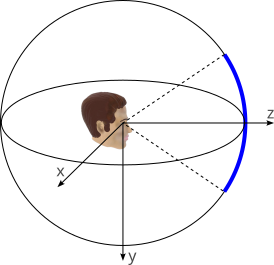
\includegraphics[width=0.30\linewidth]{fig/coordenadas.png}} \quad
	
	\subfigure[ângulos de Euler e sua representação do movimento de cabeça. \label{fig:bcs}]
	{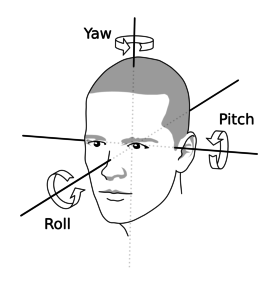
\includegraphics[width=0.30\linewidth]{fig/bcs.png}} \quad
	
	\caption{Os Sistemas de Coordenadas em um espaço cartesiano}
	\label{fig:coord_sis}
\end{figure}

Para descrever a direção da cabeça do usuário, consideramos que rodar a cabeça em uma direção é equivalente a rodar a esfera na direção oposta. Para isso, usamos um conjunto de ângulos de Euler (yaw, pitch e roll) para realizar a rotação da esfera usando a sequencia y-x-z. O yaw indica a rotação do eixo y, o pitch a rotação do eixo X e o Roll a rotação do eixo Z. Tal convenção também conhecida como angulos de Tait–Bryan é muito usado em aplicações aeroespaciais. Estes ângulos coincide com os angulos do sistema de coordenadas horizontal facilitando a identificação do centro do viewport. Sua valores são relativos à posição inicial (elevação=0 e azimute=0 no sistema horizontal, ou o vetor (0, 0, 1) no sistema cartesiano), como mostra a figura~\ref{fig:bcs}. Por se tratar de rotação, os valores dos ângulos podem assumir qualquer valor valor real (em radianos).
É convencionado que todas as rotações em sentido horário são positivas e em sentido anti-horário são negativas. Assim, olhar para cima possui um \textit{pitch} positivo, olhar para a direita possui um \textit{yaw} positivo e rodar a cabeça em sentido horário possui um \textit{roll} positivo.

A rotação de um ponto no sistema de referência (fixo) com os ângulos de Euler pode ser representada por uma equação na forma matricial $\overrightarrow{V}^T = \overrightarrow{R} \times \overrightarrow{v}^T $, onde $\overrightarrow{V}^T = (x',y',z')$ é a nova posição, $\overrightarrow{V}^T = (x,y,z)$ é o vetor no sistema de referência e $\overrightarrow{R}$ é a matriz de rotação dada pela equação~\ref{eq:matrotation}.

\begin{equation}
	R=\begin{bmatrix}
		cos(yaw) & 0 & sin(yaw)\\
		0 & 1 & 0\\
		-sin(yaw) & 0 & cos(yaw)
	\end{bmatrix}
	\begin{bmatrix}
		1 & 0 & s0\\
		0 & cos(pitch) & -sin(pitch)\\
		0 & sin(pitch) & cos(pitch)
	\end{bmatrix}
	\begin{bmatrix}
		cos(roll) & -sin(roll) & 0\\
		sin(roll) & cos(roll) & 0\\
		0 & 0 & 1
	\end{bmatrix}
	\label{eq:matrotation}
\end{equation}	
	
\subsubsection{Sistema Horizontal}

Para representar um ponto sobre a casca da esfera do vídeo, uma variação do sistema de coordenadas esféricas, chamado de sistema de coordenadas horizontal é usado como intermediário para operações entre projeções. O sistema de coordenadas horizontal, muito usado na astronomia para observação de corpos celestes, utiliza ângulos de azimute e de altitude para representar a posição de ponto na esfera em relação a um ponto de referência.

Como mostra a figura~\ref{fig:hcs}, neste sistema, o azimute é o angulo da projeção do vetor $ \overrightarrow{v}$ no plano ZX (horizonte) em relação ao eixo Z e a altitude é a elevação vertical do vetor em relação ao plano do horizonte. Por convenção, a elevação varia de -90° a 90°, sendo que o sinal positivo aponta para acima do horizonte, enquanto que o azimute varia de -180° a 180°, sendo que o sinal positivo está à direita do eixo Z. Desta forma, o pixel na posição (elevação, azimute) igual a (0,0) encontra-se no ponto (x=0, y=0, z=1). 

\begin{figure}[h]
	\centering
	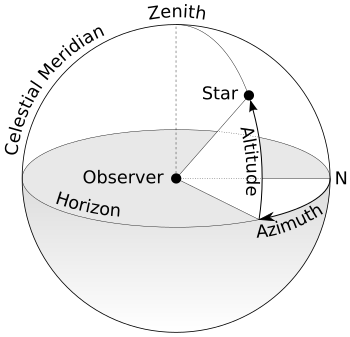
\includegraphics[width=0.30\linewidth]{fig/hcs.png}
	\caption{O Sistema de Coordenadas Horizontal}
	\label{fig:hcs}	 
\end{figure}

As equações para conversão das coordenadas cartesianas em coordenadas horizontais não dependem da projeção e podem ser descritas pelo conjunto de equações~\ref{eq:cart2hcs}.

\begin{equation}
\label{eq:cart2hcs}
\begin{split}
	\text{Azimute} &=\sin^{-1}\left(\frac{-y}{\sqrt{x^2+y^2+z^2}}\right) \\
	\text{Elevação} &=\tan^{-1}\left(\frac{x}{z}\right)
\end{split}		
\end{equation}	


\section{Projeção}

Projeções são um tipo de mapeamento entre dois espaços vetoriais. No caso, a esfera, descrita no plano cartesiano de três dimensões é mapeada em um plano bidimencional representado pela imagem. Estas técnicas são muito conhecidas no ambiente de desenvolvimento de modelagem objetos 3D em aplicações como Blender, Unreal e Unity para armazenamento de texturas em arquivos de imagem tradicionais. Ao desenhar o objeto 3D na tela, o motor gráfico busca os pixels correspondentes na imagem.

\subsubsection{Projeção Equirretangular}

A projeção equirretangular é uma técnica de mapeamento cartográfico de uma esfera para um plano retangular, preservando a proporção dos pixels, mas distorcendo a imagem. Isto é, quando mais próximo dos polos, os pixels diminuem a altura enquanto aumentam sua largura. Isto produz fortes deformações na região próxima aos polos, mas como os usuários tendem a manter o olhar a altura do horizonte, a maior parte do conteúdo do vídeo é facilmente visualizado. A figura~\ref{fig:erp} apresenta como é feita a projeção.

\begin{figure}
	\centering
	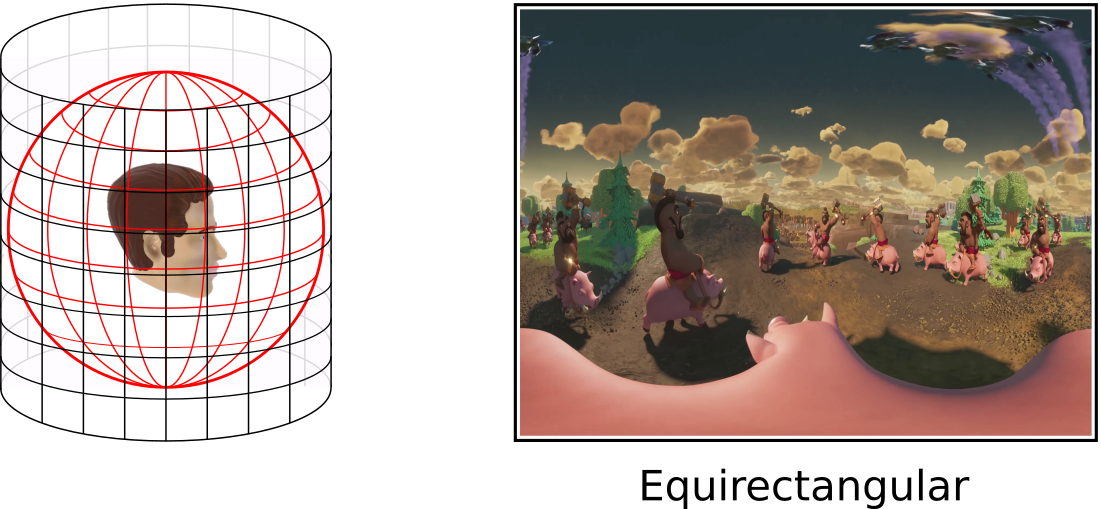
\includegraphics[width=0.8\textwidth]{fig/erp.png}
	\caption{Projeção Equirretangular mapeada no plano da imagem.}
	\label{fig:erp}
\end{figure}

No mapeamento de um vídeo 360° usando a projeção equirretangular, a esfera do vídeo é desdobrada em um plano 2D retangular, onde cada ponto na esfera é mapeado para um pixel correspondente na imagem retangular. Primeiro, a posição do pixel na esfera em coordenadas cartesianas é convertido para o sistema de coordenadas horizontal usando as equações~\ref{eq:cart2hcs}. Em seguida, as coordenadas são normalizadas em um plano uv onde u e v variam de 0 a 1, o eixo u aponta para a direita e o eixo v aponta para baixo usando as equações~\ref{eq:hcs2erp}. Por fim as coordenadas $(m, n)$ na imagem são dadas multiplicando $u$ e $v$ pela largura ($W$) e altura ($H$) da  imagem, respectivamente. O truncamento é realizado afim de se aplicar a interpolação por vizinho mais próximo.

\begin{align}
	u &= \dfrac{\text{Azimute}}{2\pi} + 0.5 \\
	v &= \dfrac{-\text{Elevação}}{\pi} + 0.5 \\
	\label{eq:hcs2erp}
\end{align}


Em seguida, a projeção é segmentada espacialmente em vídeos independentes de tamanhos iguais.
codificadores como H.265 ou AV1 transformam esta projeção em um fluxo de bits que são armazenados em arquivos contêineres como MP4. Estes arquivos podem ser armazenados ou transmitidos


\begin{table}[h]
	\centering
	\caption{Detalhes do ladrilhamento e resoluções resultantes.}
	\label{tab:ladrilhamento_resolucoes}
	\begin{tabular}{|c|p{2.5cm}|c|p{2.5cm}|c}
		\cline{1-4}
		\textbf{Ladrilhamento} & \centering\textbf{Quantidade de ladrilhos} & \textbf{Projeção} & \centering \textbf{Pixels por ladrilho} & \\ \cline{1-4}
		\multirow{2}{*}{\textbf{1x1}} & \centering\multirow{2}{*}{1} & CMP & \centering 4320x2160 & \\ \cline{3-4} 
		&   & ERP & \centering 3240x2160 & \\ \cline{1-4}
		\multirow{2}{*}{\textbf{3x2}} & \centering \multirow{2}{*}{6} & CMP & \centering 1440x1080 & \\ \cline{3-4} 
		&   & ERP & \centering 1080x1080 & \\ \cline{1-4}
		\multirow{2}{*}{\textbf{6x4}} & \centering \multirow{2}{*}{24} & CMP & \centering 720x540 & \\ \cline{3-4} 
		&   & ERP & \centering 540x540 & \\ \cline{1-4}
		\multirow{2}{*}{\textbf{9x6}} & \centering \multirow{2}{*}{54} & CMP & \centering 480x360 & \\ \cline{3-4} 
		&   & ERP & \centering 360x360  & \\ \cline{1-4}
		\multirow{2}{*}{\textbf{ 12x8}} & \centering \multirow{2}{*}{96} & CMP & \centering 360x270 & \\ \cline{3-4} 
		&    & ERP & \centering 270x270 & \\ \cline{1-4}
	\end{tabular}
\end{table}


As projeções mais comuns são a projeção equirretangular (ERP) e projeção cubemap (CMP)., encapsulados em arquivos MP4, por exemplo e armazenados ou transmitidos pela rede. Desta forma, para poder manipular os pixels no domínio da projeção e da esfera, extrair o viewport e calcular a qualidade do vídeo, foi necessário desenvolver uma nova biblioteca chamada video360tools\footnote{https://github.com/henriquedgarcia/video360utils} que realiza o mapeamento ente diferentes sistemas coordenadas para as projeções equirretangular e cubemap. Para isto foi definido a relação entre os sistemas de coordenadas cartesiano, horizontal e sistema de coordenadas de corpo conforme descrito a seguir.



\subsubsection{Projeção Cubemap}

A projeção cubemap é outra técnica comumente usada em vídeos 360° para mapear um ambiente tridimensional em uma representação bidimensional, atualmente adotado pelo Youtube e pelo Facebook. Ao contrário da projeção equirretangular, que mapeia a esfera em um plano retangular, a projeção cubemap mapeia a esfera em seis faces quadradas de um cubo de lado igual a 2. As seis faces correspondem a visão ao redor do ponto de captura. As faces geralmente são organizadas em uma grade de 3x2 formando um único arquivo de imagem. As três imagens superiores são as faces da esquerda, frente e direita, Enquanto as faces de baixo são rotacionadas 90° em sentido horário e correspondem as faces de cima, de trás e de baixo. A figura~\ref{fig:cmp} mostra um exemplo de mapeamento para projeção Cubemap (CMP).

\begin{figure}
	\centering
	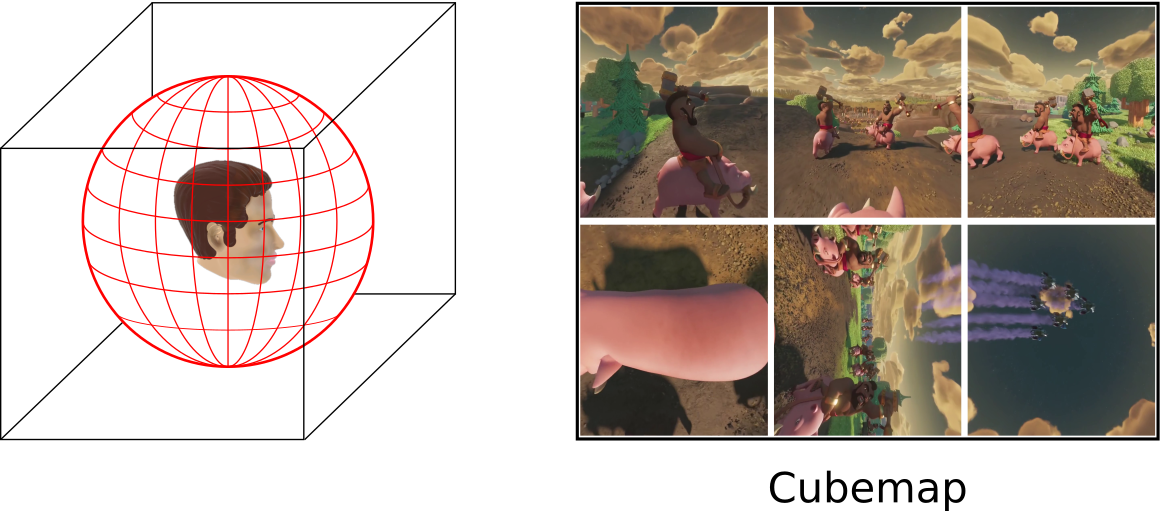
\includegraphics[width=0.8\textwidth]{fig/cmp.png}
	\caption{Projeção Cubemap e a disposição das seis faces no plano da imagem.}
	\label{fig:cmp}
\end{figure}

Como forma de representação auxiliar, cada face é mapeada em um plano $uv$ conforme a tabela~\ref{tab:uv_erp}, onde as coordenadas $u$ e $v$ variam de -1 a +1, com $u$ apontando para direita e $v$ apontando para baixo. Por fim, as coordenadas $uv$ são convertidas para posições dos pixels pela equação $ (uv+1)\times \frac{A}{2}-0.5$, onde A é o número de pixels em uma face do quadrado, e reposicionado na imagem. O processo inverso, de mapeamento do plano uv para o espaço cartesiano é feito pela tabela~\ref{tab:uv_erp}.

\begin{table}[htbp]
	\centering
	\caption{Tabela de coordenadas $(X, Y, Z)$ em função de $(U, V)$}
	\label{tab:uv_erp}
	\begin{tabular}{|c|c|c|c|}
		\hline
		\textbf{Face} & \textbf{X} & \textbf{Y} & \textbf{Z} \\
		\hline
		0 & $-1.0$ & $v$    & $u$    \\
		1 & $u$    & $v$    & $1.0$  \\
		2 & $1.0$  & $v$    & $-u$   \\
		3 & $-u$   & $1.0$  & $v$    \\
		4 & $-u$   & $v$    & $-1.0$ \\
		5 & $-u$   & $-1.0$ & $-v$   \\
		\hline
	\end{tabular}
\end{table}

\begin{table}[htbp]
	\centering
	\caption{Tabela de condições e valores de \( face, u, v \) em função de $(X, Y, V)$}
	\label{tab:condicoes}
	\begin{tabular}{|c|c|c|c|}
		\hline
		\textbf{Condição} & \textbf{Face} & \textbf{u} & \textbf{v} \\
		\hline
		$ |X| \geq |Z|  \text{ e }  |X| \geq |Y|  \text{ e }  X < 0 $ & 0 &  $\frac{Z}{|X|}$ & $ \frac{Y}{|X|} $ \\
		$ |Z| \geq |X|  \text{ e }  |Z| \geq |Y|  \text{ e }  Z > 0 $ & 1 &  $\frac{X}{|Z|}$ & $ \frac{Y}{|Z|} $ \\
		$ |X| \geq |Z|  \text{ e }  |X| \geq |Y|  \text{ e }  X > 0 $ & 2 &  $\frac{-Z}{|X|}$  & $ \frac{Y}{|X|} $ \\
		$ |Y| \geq |X|  \text{ e }  |Y| \geq |Z|  \text{ e }  Y < 0 $ & 3 &  $\frac{-X}{|Y|} $ & $ \frac{Z}{|Y|} $ \\
		$ |Z| \geq |X|  \text{ e }  |Z| \geq |Y|  \text{ e }  Z < 0 $ & 4 &  $\frac{-X}{|Z|}$  & $ \frac{Y}{|Z|} $ \\
		$ |Y| \geq |X|  \text{ e }  |Y| \geq |Z|  \text{ e }  Y > 0 $ & 5 &  $\frac{-X}{|Y|}$  & $ \frac{-Z}{|Y|} $ \\
		\hline
	\end{tabular}
\end{table}


\subsection{O Viewport}

O viewport é definido como a porção da esfera que é visível pelo usuário. Como a visão humano (FOV -\textit{ Field of View}) é limitada, os HMD reproduzem um FOV de aproximadamente $120^\circ\times90^\circ$. Para isto os ponto da esfera que pertencem ao viewport são projetados a um plano tangente a esfera no ponto $ P(0, 0, 1) $ utilizando a projeção Gnomônica ou Retilínea\footnote{https://www.wolframalpha.com/input?i=rectilinear+projection}, como pode ser visto na figura~\ref{fig:projecao_viewport}. 

\begin{figure}[htb]
        \centering
        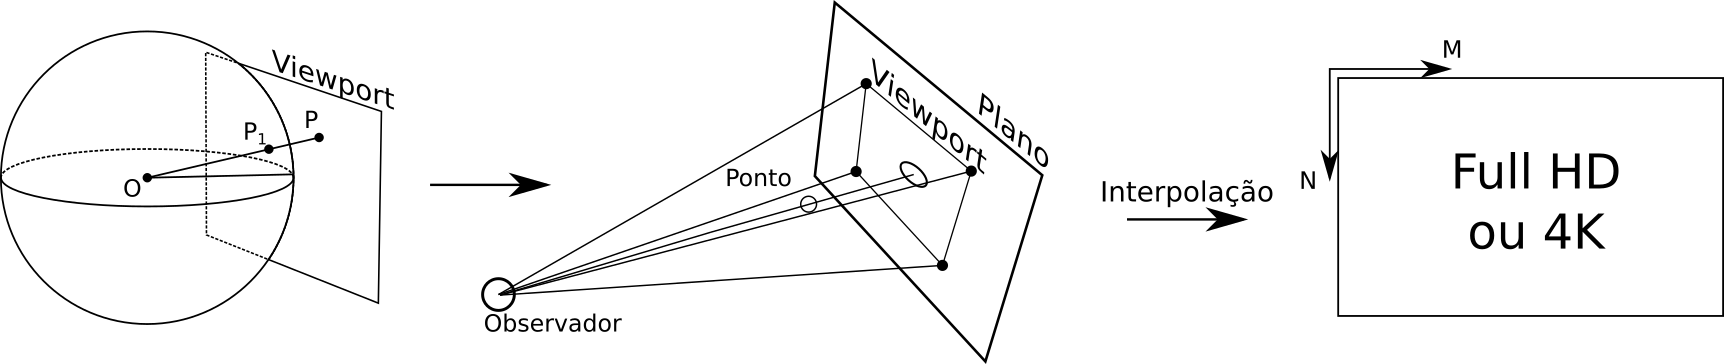
\includegraphics[width=1.0\linewidth]{fig/projecao_viewport.png}
        \caption{Extração do viewport usando projeção retilinear ou gnomônica.}
        \label{fig:projecao_viewport}
\end{figure}

Primeiramente, a matriz da imagem do viewport é pre alocada de acordo com a resolução exibida para o usuário. Em vez do valor do pixel, cada célula da matriz é preenchida com a posição do pixel na esfera usando coordenadas horizontais, de $-fov_X$ a $+fov_X$ e de $-fov_Y$ a $+fov_y$. Em seguida, cada coordenada é convertida para o sistema cartesiano usando as equações~\ref{eq:cart2hcs}. Finalmente as coordenadas cartesianas são convertidas para o domínio da projeção, seja equirretangular ou cubemap. Obviamente os pontos não serão os mesmos, então é usado algum método de interpolação, com interpolação por vizinho mais próximo ou interpolação linear. Agora basta mapear os pixels do viewport com os pixels da projeção.

Por outro lado, para verificar quais ladrilhos pertencem ao viewport, é preciso verificar se um pixel da projeção está sendo visualizado. Para isto, consideramos que o viewport compreende o espaço interno da intersecção de quatro planos que passam pelo centro da esfera e possuem inclinação relativas ao FOV do viewport e ao eixo Z. Por exemplo, um FOV de $ 120^\circ\times 90^\circ $ está limitado a 60° à direita e -60° à esquerda do eixo Z e 45° acima e -45° abaixo do eixo Z. Estes planos definem os limites superiores, inferiores, esquerdo e direito do viewport. Estas normais devem apontar para o lado de fora do viewport, assim o viewport compreende apenas os pontos que estão abaixo de todos os planos ao mesmo tempo. As normais que definem os planos são descritas na equação~\ref{eq:normals}, onde $fov_X$ e $fov_Y$ são os ângulos horizontal e vertical do FOV, respectivamente.

\begin{align}
        N &=\begin{bmatrix}
                0 & -cos\left(\dfrac{fov_Y}{2}\right) & -sin\left(\dfrac{fov_Y}{2}\right) \\
                0 & sin\left(\dfrac{fov_Y}{2}\right) & -cos\left(\dfrac{fov_Y}{2}\right) \\
                cos\left(\dfrac{fov_X}{2}\right) & 0 & -sin\left(\dfrac{fov_X}{2}\right)\\
                -sin\left(\dfrac{fov_X}{2}\right) & 0 & -cos\left(\dfrac{fov_X}{2}\right)
        \end{bmatrix}
        \label{eq:normals}
\end{align}

Após o movimento de cabeça, as normais são rotacionadas de acordo com as coordenadas de corpo $H(yaw, pitch, roll)$ e assumem nova posição $ N_R $ dado pelo produto matricial do vetor de normais com a matriz de rotação $ N_R = \textbf{N} \times \textbf{R}$. Um pixel $ \textbf{P}$ qualquer no espaço cartesiano pertencerá ao viewport se o produto interno $ N.T \dot P <=0 $ para todas as normais, ou seja, estão abaixo das normais após as normais forem rotacionadas durante o movimento da cabeça.

\section{Qualidade objetiva do vídeo}

\subsection{Qualidade para o cliente}
No processo de preparação para o \textit{streaming} de vídeos esféricos, a esfera de vídeo passa por um mapeamento em um plano, introduzindo distorções que variam ao longo do plano. Ao utilizar métodos de compressão com perda, os codificadores geralmente aplicam a quantização de forma uniforme em todo o quadro, podendo impactar mais severamente em regiões distorcidas pela projeção. Após a decodificação, os pixels renderizados são remapeados de volta para a esfera, e quaisquer artefatos de codificação, como blocados, aliasing, efeito de \textit{Gibbs}, borrado, etc, também serão distorcidos.

Assim, a qualidade objetiva da viewport é definida como a disparidade entre o viewport extraído do vídeo codificado e o viewport de um vídeo de referência.   A Figura~\ref{fig:QualityWorkflow} ilustra como medir a qualidade objetiva do \textit{viewport}, considerando a esfera sem degradação e a esfera recuperada após a compressão. A viewport precisa ser extraída com base na posição da cabeça do usuário em ambos os vídeos de referência e codificado, assim o MSE e SSIM devem ser calculados entre esses quadros. O MSE foi usado no lugar do PSNR, pois o PSNR deve ser calculado apenas após o cálculo da média do MSE de todos os quadros de um vídeo, como mostra a documentação do filtro de PSNR do ffmpeg\footnote{https://ffmpeg.org/ffmpeg-filters.html}. As operações de cálculo MSE e do SSIM foram calculadas usando a biblioteca scikit-image. Apesar do MSE e o SSIM falhem ao tentar medir qualidade sob certas condições, elas são suficientes para se medir distorções produzidas por artefatos esperados como bordas de ladrilho, borrado e blocado.~\cite{Bovik2009} 

\begin{figure}[ht]
        \centering
        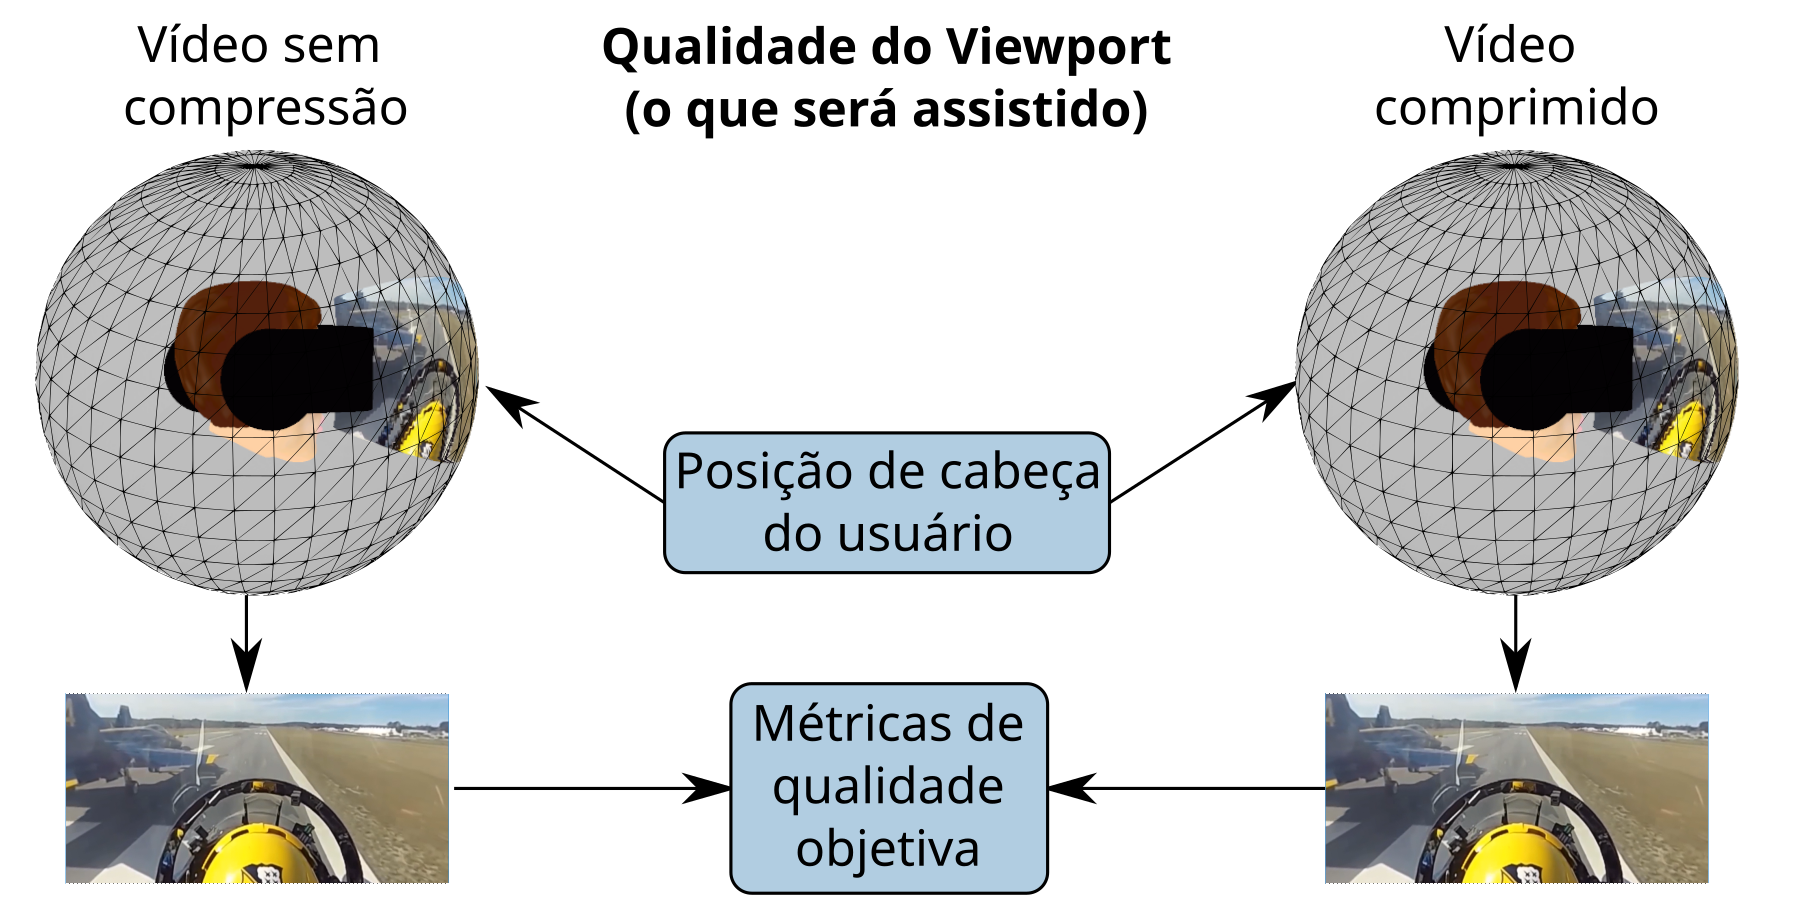
\includegraphics[width=0.8\linewidth]{fig/Project_Quality_Workflow_2.png}
        \caption{Avaliação de qualidade objetiva do viewport.}
        \label{fig:QualityWorkflow}
\end{figure}

Quando o vídeo é segmentado em ladrilhos, é necessário reconstruir a projeção com os ladrilhos que são visualizados durante todo o período de duração de um \textit{chunk}. Como o usuário está movimentando a cabeça, durante um \textit{chunk} os ladrilhos vistos podem se modificar. Para o DASH o \textit{chunk} inteiro precisa estar no \textit{buffer} do cliente para que apenas alguns quadros possam ser decodificados. A aplicação cliente precisa saber de antemão quais ladrilhos serão vistos e então solicitá-los ao servidor. Por exemplo, na figura~\ref{fig:selectTiles} vemos uma projeção equirretangular segmentada em 3x3 ladrilhos. No instante 0 o usuário está visualizando os ladrilhos 3, 4, 6, 7 e 8, porém, devido ao movimento da cabeça, antes de se concluir a reprodução do \textit{chunk}, o usuário passa a ver os ladrilhos 0, 1, 3, 4, 6 e 7. Os ladrilhos 0 e 1 passaram a ser vistos e o ladrilho 8 deixou de ser visto. Os ladrilhos 0 e 1 precisam já ter sido baixados e decodificados para que o usuário veja seu conteúdo nos instantes finais do \textit{chunk}.

\begin{figure}[h]
        \centering
        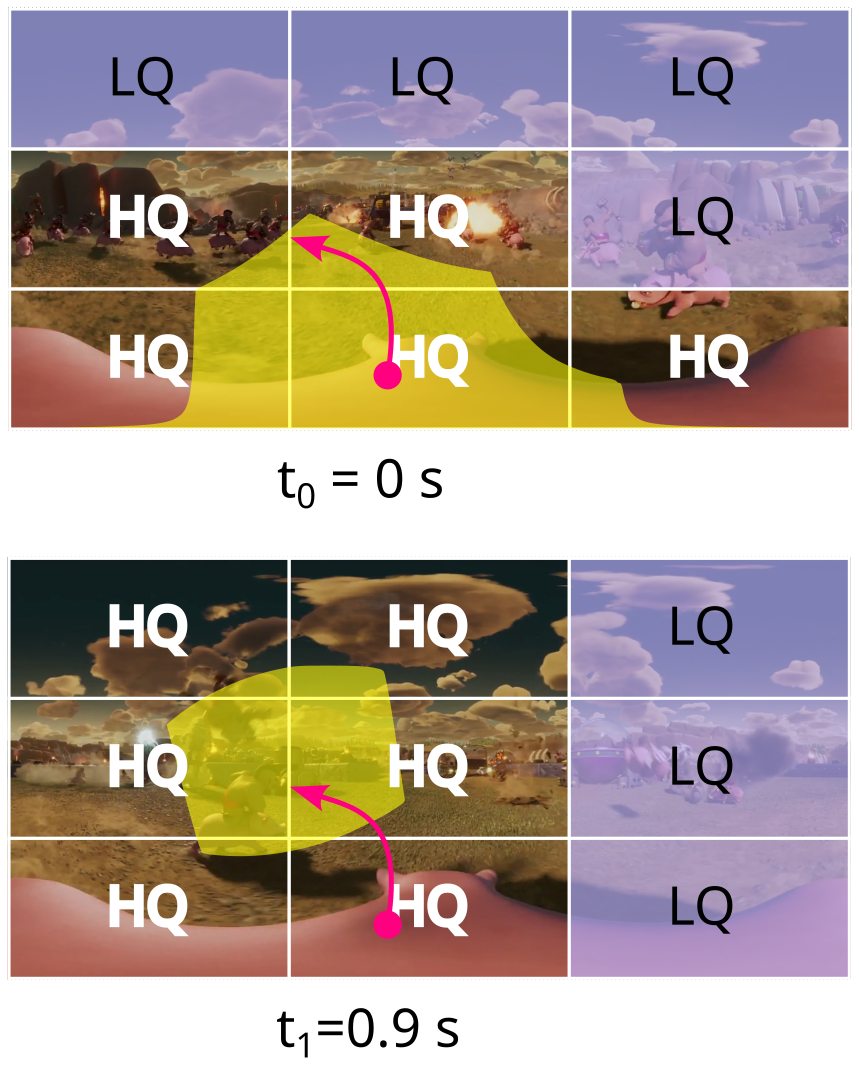
\includegraphics[width=0.5\linewidth]{fig/Streaming of Tiles 2.png}
        \caption{Tiles que deverão ser solicitados ao servidor e que serão assistidos durante um \textit{chunk}.}
        \label{fig:selectTiles}
\end{figure}

Em um cenário com decodificadores operando em paralelo o tempo para a decodificação dos chunks do viewport será igual ao maior tempo de decodificação entre todos os tiles selecionados. Porém, em um ambiente com threads simples, o tempo de decodificação será igual a soma de todos os tempos de decodificação. A taxa de bits necessária para a reprodução do viewport será igual soma de todos os ladrilhos que foram visualizados durante a duração de um chunk.

\subsection{Qualidade para o servidor}

Por outro lado, para sistemas de transmissão adaptativos como o MPEG DASH, a qualidade do vídeo codificado está diretamente correlacionada com sua taxa de bits. Esta correlação baseia-se no pressuposto de que uma taxa de bits mais elevada corresponde a uma melhor qualidade. A lógica por trás dessa relação reside no fato de que a qualidade medida, normalmente avaliada usando métricas como PSNR ou MSE, quantifica o erro induzido pela quantização no processo de compressão com perdas. Neste contexto, o aumento da quantização leva a uma perda de detalhes e a uma maior compressão, reduzindo a qualidade e também a taxa de bits.

No entanto, é importante notar que as métricas SSIM e PSNR podem não ser adequadas para avaliar diretamente a qualidade da projeção, especialmente considerando as distorções introduzidas durante o processo de projeção. Consequentemente, métricas de qualidade esféricas foram desenvolvidas para avaliar o nível objetivo de qualidade de uma projeção. A parte superior da Figura \ref{fig:QualityDiagram} ilustra como a “qualidade objetiva da projeção” deve ser medida. Métricas de qualidade devem ser aplicadas entre a projeção antes da codificação (vídeo de referência) e a projeção decodificada após a compressão (vídeo degradado).

\begin{figure}[htb]
        \centering
        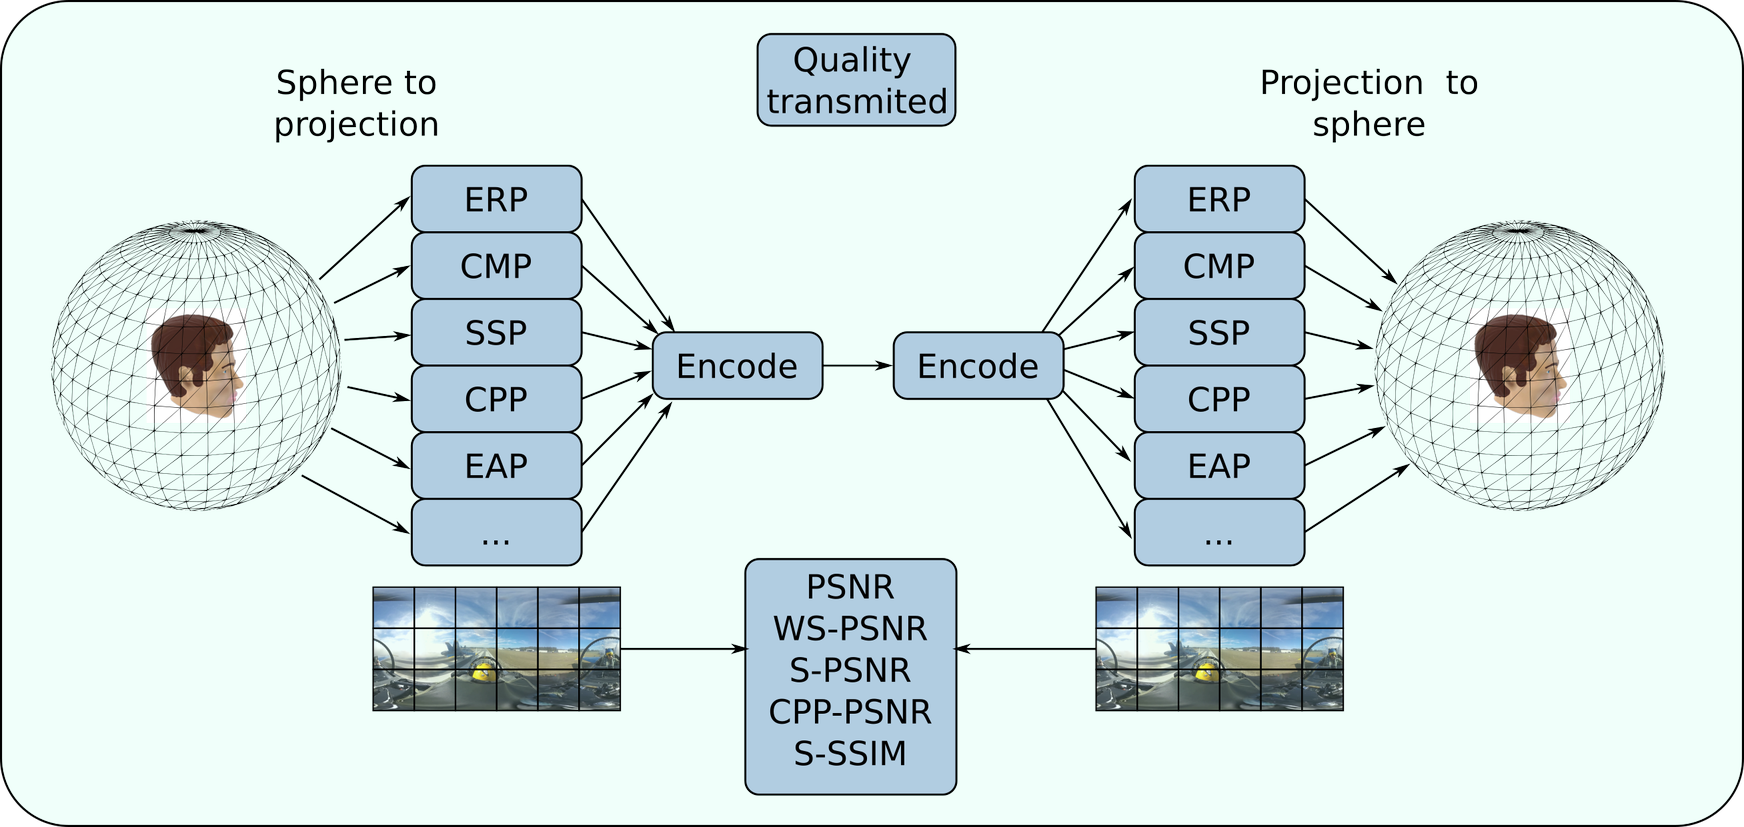
\includegraphics[width=0.7\linewidth]{fig/diagrama e qualidade 1.png}
        \caption{Avaliação de qualidade objetiva da projeção.}
        \label{fig:QualityDiagram}
\end{figure}

Conseguir um vídeo codificado de qualidade alta requer minimizar as perdas a um nível que não seja perceptível o suficiente para causar desconforto. A qualidade objetiva da projeção é definida especificamente como a disparidade entre o vídeo codificado e o vídeo de referência da perspectiva da projeção. Consequentemente, a qualidade objectiva da projeção de vídeo difere da qualidade objetiva da janela de visualização. O que os algoritmos convencionais de taxa de bits adaptativa (ABR) podem considerar satisfatório no domínio de codificação/transmissão pode não estar necessariamente alinhado com a qualidade ideal no domínio da esfera.

Para formular um algoritmo eficaz de adaptação de taxa de bits (ABR) adaptado para streaming de vídeo em 360°, é necessário um estudo aprofundado para compreender a relação entre a qualidade da janela de visualização e a qualidade da projeção. Esse mapeamento torna-se crucial no processo de tomada de decisão para troca de qualidade, reconhecendo que o usuário e o algoritmo ABR operam em planos distintos~\cite{tran2017, Xu2020}.

\subsubsection{MSE/PSNR}

PSNR, ou \textit{Peak Signal-to-Noise Ratio}, e o MSE (\textit{Mean Squared Error}) são métricas amplamente utilizada para avaliar a qualidade de imagens e vídeos reconstruídos ou compactados. Quantifica a relação entre a potência máxima possível de um sinal (neste contexto, uma imagem ou vídeo) e a potência do ruído corruptor que impacta a qualidade do sinal. As duas métricas se relacionam através da seguinte fórmula:

\begin{align}
        \label{MSE}
        MSE&= \frac{1}{M\times N}\sum^{M-1}_{i=0}\sum^{N-1}_{j=0} \left(y(i,j) - y'(i,j)\right)^2 \\
        \label{PSNR}
        PSNR&=10 \times \log_{10}\left(\frac{MAX^2_I}{MSE}\right)
\end{align}

Primeiro, o MSE é calculado para todos os quadros do vídeo e, no final da reprodução, a média do MSE é usado para calcular o PSNR (\textit{Peak Signal-to-Noise Ratio}). Para um vídeo segmentado em ladrilhos, considere que $L_{quadro} $ é a lista de quadros tocados pelo viewport ao longo da reprodução do vídeo e $MSE_{frame}(i)$ é o MSE de um quadro. A qualidade de uma seção de vídeo assistido pelo usuário, é definida pelo PSNR utilizando a média do MSE de todos quadros que aparecerem no viewport, como mostra a equação~\ref{eq:agerage_MSE}.

\begin{equation}
        \bar{MSE} = \sum^{N_{frames}}_{i=0} \dfrac{MSE_{frame}(i)}{N_{frames}}
        \label{eq:agerage_MSE}
\end{equation}

\subsubsection{S-MSE/S-PSNR}

O S-PSNR emprega uma lista de 655.362 pontos equidistantes na esfera para identificar os pixels correspondentes na projeção original e na projeção degradada para em seguida calcular o MSE para todos estes pontos. Este processo é ilustrado na Figura~\ref{fig:spsnr}. Encontra-se o ponto na projeção correspondente ao ponto da esfera e então calcula-se o erro. Desta forma é possível comparar duas projeções diferentes. Apesar desta métrica se preocupar em uniformizar as amostras no domínio da esfera, onde o usuário realmente interage, quanto maior a resolução da projeção, mais pixels serão desprezados no cálculo da métrica.

\begin{figure}[h]
        \centering
        \subfigure[O S-PSNR busca os pixels na projeção de referência ``R'' e a projeção degradada ``T'' correspondentes aos pontos ``S'' pré-definidos e equidistantes na esfera.\label{fig:spsnr}]{
                \quad
                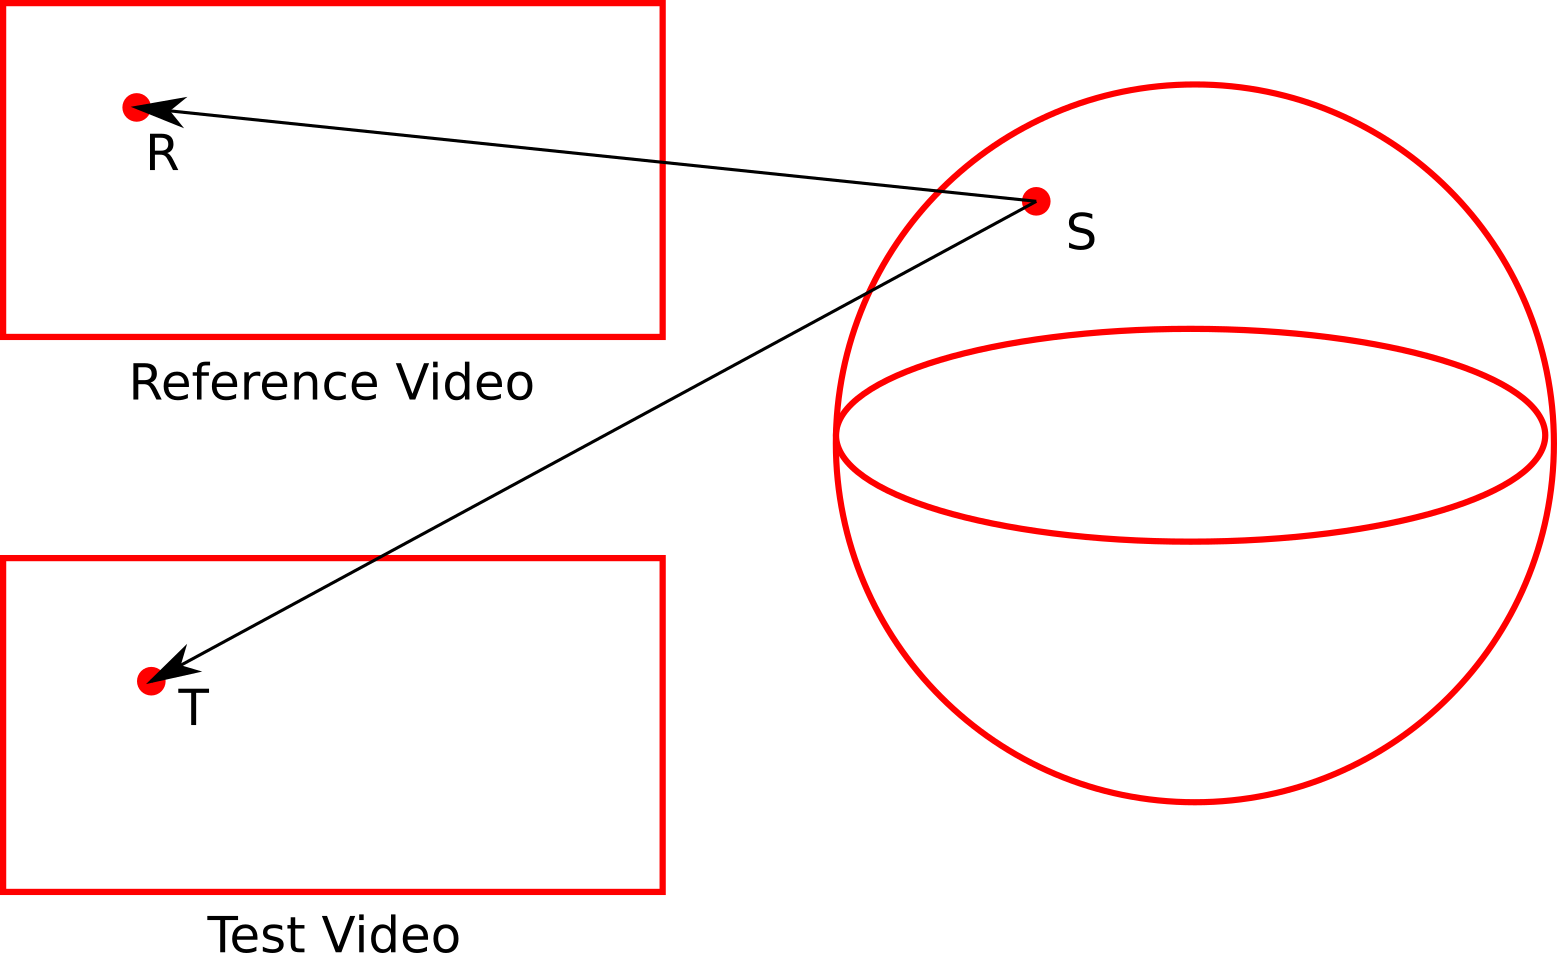
\includegraphics[width=0.4\linewidth]{fig/diag_spsnr.png}
                \quad
        }
        \quad
        \subfigure[Mapa de pesos para a projeção Equirretangular e Cubemap usado pela métrica WS-MSE\label{fig:wspsnr}]{
                \quad\quad
                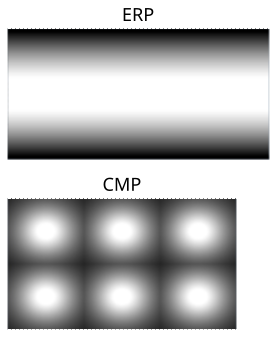
\includegraphics[width=0.25\linewidth]{fig/ws-psnr.png}
                \quad\quad
        }     
\end{figure}

\subsubsection{WS-MSE/WS-PSNR}

O WS-MSE e o WS-PSNR incorporam pesos para cada pixel da projeção ao calcular MSE, conforme expresso nas Equações \ref{eq:WMSE} e \ref{eq:WS-PSNR}. Considerando uma projeção com resolução MxN, o WS-MSE primeiro calcula a média ponderada do quadrado das diferenças dos pixels y e y' na posição (i,j) para todos os pixels de cada quadro. O cálculo do WS-PSNR só é aplicado sobre a média do WS-MSE de todos os quadros.

\begin{align}
        \label{eq:WMSE}
        MSE&= \frac{\sum^{M-1}_{i=0}\sum^{N-1}_{j=0} \left(y(i,j) - y'(i,j)\right)^2 \times w(i,j)}{\sum^{M-1}_{i=0} \sum^{N-1}_{j=0} w(i,j)}\\[12pt]
        \label{eq:WS-PSNR}
        WS\mbox{-}PSNR&=10 \times \log_{10}\left(\frac{MAX^2_I}{MSE}\right)
\end{align}

Os pesos de cada pixel dependem da sua posição na projeção e do tipo de projeção. Projeções como ERP esticam mais os polos enquanto a projeção Cubemap distribui as faces na imagem de forma arbitrária. As equações \ref{eq:w_wpsnr1} e \ref{eq:w_wpsnr2} delineiam os pesos para as projeções equirretangular (ERP) e cubemap (CMP). No caso de uma projeção Cubemap, considera-se que todas as faces do cubo são quadradas e possuem resolução $A \times A$. O resultado pode ser visto na figura~\ref{fig:wspsnr}

\begin{align}
        \label{eq:w_wpsnr1}
        w_{ERP}(i,j)&=cos\left(\frac{(j+0.5-N/2)\pi}{N}\right) \\
        \label{eq:w_wpsnr2}
        w_{CMP}(i,j)&=\left(1 + \frac{d^2(i,j)}{r^2}\right)^{\frac{-3}{2}} \\
        d^2(i, j)&=(i+0.5-\dfrac{A}{2})^2 +(j+0.5-\dfrac{A}{2})^2
\end{align}

\subsection{Estatísticas}

Determinar as estatísticas das métricas é muito importante afim de entender seu comportamento e distribuição ao longo da reprodução para diferentes tipos de conteúdos. A distribuição das métricas de tempo de decodificação, taxa de bits e qualidade objetiva foram analisadas considerando que as distribuições são positivas e contínuas, descartando distribuições discretas e distribuições sobre a reta real. Considerando também as distribuições disponíveis nos pacotes estatísticos mais comuns, como SciPy e Matlab, as distribuições analisadas são: Burr Tipo XII , Birnbaum-Saunders, Gamma, Inversa Gaussiana, Rayleigh, Log Normal, Generalized Pareto, Pareto, Half-Normal, e Exponencial. O processo de ajuste mais comum se baseia na estimação dos parâmetros por máxima verossimilhança e para a avaliação das distribuições foi utiliza o erro quadrático médio (RMSE).

A correlação entre as métricas é feita entre todos os chunks de cada ladrilho. Como a correlação mede a dependência entre duas variáveis e as métricas variam de forma diferente para cada tipo de ladrilhamento e para cada qualidade de codificação, a correlação deve ser medida considerando apenas as ladrilhos de uma mesma qualidade e de uma mesma região de cada vídeo. Assim, as métricas de 60 chunks para cada ladrilho, para cada qualidade e para cada vídeo puderam ser correlacionada. Por fim a média de todas as correções são consideradas ao se comparar diferentes cenários.


\chapter{Avaliação e resultados}\label{Cap:Evaluation}

Para otimizar o streaming de vídeo esférico é essencial conhecer suas principais características que afetam seu desempenho e sua qualidade. Para caracterizar o tráfego de vídeo panorâmico de 360 graus ladrilhado com DASH-SRD, é essencial replicar as condições de transmissão, codificação e segmentação do vídeo durante uma seção do cliente. Além disso, as métricas de avaliação devem ser relacionadas a experiência do usuário e do servidor. Para o cliente o queremos medir o tempo de decodificação, a taxa de bits e a qualidade do vídeo exibido no viewport. Para o servidor, queremos que a melhor qualidade seja entregue com a menor taxa de bits possível e para isso avaliamos métricas de qualidade de codificação tradicional e de vídeo esférico e sua correlação com o a taxa de bits.

Em um sistema de streaming adaptativo como DASH, os chunks do vídeo devem ser codificado de forma que possa ser decodificado de forma independente do chunk anterior, isto é, não tenham dependência temporal. Para isso, o GOP (\textit{Group of pictures}) usado em codificação preditiva, precisa ser do tipo fechado e com o numero de quadros fixo igual a duração do \textit{chunks}. Além disso, para evitar que haja artefatos nas bordas dos ladrilhos durante a reprodução, os ladrilhos precisam ser codificados de forma que a qualidade seja aproximadamente a mesma entre todos os ladrilhos de um quadro ao longo de sua reprodução. Geralmente os vídeos que serão transmitidos devem ser codificados baseado em taxa média para que o buffer de reprodução possa ser facilmente modelado. Porém, se o vídeo for segmentado em ladrilhos, cada ladrilho possuirá uma complexidade diferente, por exemplo, ladrilhos que mapeiam o topo ou a base da esfera tendem a retratar o chão ou o céu, que possuem poucos detalhes, sendo assim a compressão é alta, mesmo usando pouca quantização. Por outro ladro, ladrilhos que mapeiam regiões da esfera com alta atividade temporal e espacial, como movimento, pessoas, texturas, etc, tentem a ser difícil de comprimir. Assim, os ladrilhos de um vídeos não devem possuir a mesma taxa de bit, mas sim a mesma distorção de codificação. Em contra partida, a taxa de bits poderá variar muito dependendo do conteúdo do vídeo, inserindo mais complexidade na modelagem do buffer de reprodução.


\section{Caracterização dos elementos do servidor}

O fluxo de trabalho da caracterização é visto na figura~\ref{fig:fluxograma1}. Os vídeos selecionados São os mesmos empregados no estudo de Nasrabadi~\cite{Nasrabadi2019}. Seis vídeos foram gravados pessoalmente pelo autor em projeção equirretangular. Os demais vídeos foram obtidos do YouTube em projeção cúbica. O processo de download foi executado usando a ferramenta JDownloader\footnote{https://jdownloader.org/} e, devido a variabilidade de qualidades e formatos abrangendo da plataforma, demos preferência a vídeos codificados com h.264, resolução de 4K e 30 fps (quadros por segundo). Apesar disto, os vídeos estavam em duas projeções diferentes e possuíam grande variabilidade de resoluções e taxas de quadro. Isto nos levou a padronizá-los afim de podermos comparar suas características. 

\begin{figure}
        \centering
        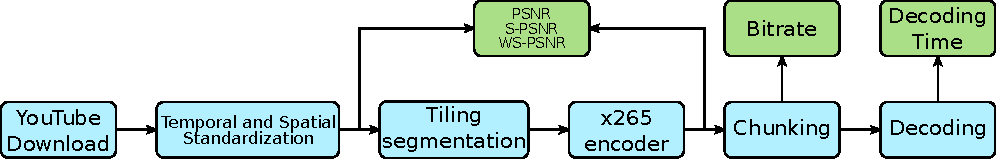
\includegraphics[width=0.7\linewidth]{fig/Fluxograma1.pdf}
        \caption{Fluxograma para captura de métricas de desempenho.}
        \label{fig:fluxograma1}
\end{figure}

Assim, topos os vídeos foram convertidos para as projeções cubemap e equirretangular usando o codificador de referência HM 16.9 com a biblioteca 360lib da MPEG\footnote{https://jvet.hhi.fraunhofer. de/svn/svn\_360Lib/}. Em seguida, convertidos para as resoluções $3240\times2160$ (CMP) e $4320\times2160$ (ERP), com taxa de quadros igual a 30 fps. A proporção da projeção foi definida dependendo da projeção utilizada. Para a projeção equirretangular, a proporção é de 2:1, pois ela mapeia os 360° em torno da esfera e os 180° de polo a polo. Já a projeção cúbica apresenta uma proporção de 3:2, pois cada uma das seis faces do cubo é projetada a 90° tanto na latitude quanto na longitude. Por questões práticas, os vídeos foram comprimidos sem perda usando codificador x265 do ffmpeg com CRF igual a 0 e armazenados em arquivos mp4.

A Tabela~\ref{tab:list_videos} exibe a lista dos cinquenta e seis vídeos utilizados. Os vídeos estão codificados com CRF 28 com a configuração padrão do codificador x265. Conforme estudo de Nasrabadi, os vídeos foram classificados de acordo com o movimento da câmera e o numero de objetos na cena. O número de objetos na cena foram definidos pelo autor. O valor da coluna "Grupo" é composto pela primeira inicial do tipo de movimento de câmera (fixo, horizontal, vertical, rotacional, múltiplo) e numero de objetos na cena (nenhum, simples, múltiplo). Assim, o grupo "VM" corresponde ao movimento Vertical com Múltiplos objetos.

\begin{longtable}{|c|c|c|c|c|c|c|}
        \caption{Vídeos usados no experimento}
        \label{tab:list_videos} 
        \\
        
        \hline
        Câmera & Objetos & Nome & Projeção & SI & TI  &  \makecell{Taxa de \\ Bits (Mbps)} \\
        \hline
        \endfirsthead
        
        \multicolumn{7}{c}%
        {{\bfseries \tablename\ \thetable{} -- Continuação da página anterior}} \\
        \hline
%        Grupo & Nome & Projeção & SI & TI  &  \makecell{Taxa de \\ Bits (Mbps)} \\
        Câmera & Objetos & Nome & Projeção & SI & TI  &  \makecell{Taxa de \\ Bits (Mbps)} \\
        \hline
        
        \endhead
        
        \multicolumn{7}{|r|}{{Continua na próxima página}} \\ \hline
        \endfoot
        
        \hline
        \endlastfoot
        
        
        \multirow{12}{*}{Fixo} & \multirow{4}{*}{Nenhum} & \multirow{2}{*}{montana} & ERP &  33.4 &   0.34 &   3.033 \\  \cline{4-7}
                               &                         &                          & CMP &  35.7 &   0.19 &   2.811 \\  \cline{3-7}
                               &                         & \multirow{2}{*}{sunset}  & ERP &  15.6 &   0.44 &   1.571 \\ \cline{4-7}
                               &                         &                          & CMP &  18.7 &   0.46 &   1.442 \\ \cline{2-7}
        
                               & \multirow{4}{*}{Simples}& \multirow{2}{*}{closet\_tour}  & ERP &  51.0 &   1.65 &   2.349 \\ \cline{4-7}
                               &                         &                                & CMP &  57.2 &   1.95 &   2.276 \\ \cline{3-7}
                               &                         & \multirow{2}{*}{video\_04}     & ERP &  49.9 &   1.19 &   2.875 \\ \cline{4-7}
                               &                         &                                & CMP &  50.9 &   1.11 &   2.245 \\ \cline{2-7}
        
                               & \multirow{4}{*}{Multi} & \multirow{2}{*}{dubstep\_dance}   & ERP &  32.9 &   6.14 &   2.771 \\ \cline{4-7}
                               &                        &                                   & CMP &  38.0 &   6.28 &   2.516 \\ \cline{3-7}
                               &                        & \multirow{2}{*}{rhinos}           & ERP &  38.5 &   0.71 &   3.799 \\ \cline{4-7}
                               &                        &                                   & CMP &  39.8 &   0.63 &   3.251 \\ \hline
                                 
        \multirow{12}{*}{Horizontal} & \multirow{4}{*}{Nenhum} & \multirow{2}{*}{drone\_footage}   & ERP &  30.3 &   5.49 &   5.153 \\ \cline{4-7}
                                     &                         &                                   & CMP &  37.2 &   5.80 &   4.334 \\ \cline{3-7}
                                     &                         & \multirow{2}{*}{petite\_anse}     & ERP &  41.4 &   7.84 &   5.913 \\ \cline{4-7}
                                     &                         &                                   & CMP &  39.4 &   7.50 &   4.919 \\ \cline{2-7}
                                 
                               & \multirow{4}{*}{Simples} & \multirow{2}{*}{cable\_cam}        & ERP &  49.7 &  17.54 &  18.790 \\ \cline{4-7}
                               &                      &                                    & CMP &  53.1 &  18.47 &  17.554 \\ \cline{3-7}
                               &                      & \multirow{2}{*}{motorsports\_park} & ERP &  35.6 &   8.15 &   3.545 \\ \cline{4-7}
                               &                      &                                    & CMP &  41.7 &   8.88 &   3.413 \\ \cline{2-7}
                                 
                               &  \multirow{4}{*}{Multi} & \multirow{2}{*}{chariot\_race}    & ERP &  39.1 &  16.87 &   8.034 \\ \cline{4-7}
                               &                       &                                   & CMP &  44.8 &  18.99 &   7.519 \\ \cline{3-7}
                               &                       & \multirow{2}{*}{nyc\_drive}       & ERP &  82.7 &  24.59 &  12.176 \\ \cline{4-7}
                               &                        &                                  & CMP &  92.7 &  27.72 &  11.565 \\ \hline
                                 
        \multirow{8}{*}{Vertical} &  \multirow{4}{*}{Nenhum} & \multirow{2}{*}{elevator\_lift}   & ERP &  52.9 &   8.46 &   2.325 \\ \cline{4-7}
                                  &                       &                                   & CMP &  60.3 &   9.59 &   2.100 \\ \cline{3-7}
                                  &                       & \multirow{2}{*}{glass\_elevator}  & ERP &  74.6 &   9.08 &   5.432 \\ \cline{4-7}
                                  &                       &                                   & CMP &  82.1 &  11.82 &   5.974 \\ \cline{2-7}
                                 
                                  &  \multirow{4}{*}{Multi} & \multirow{2}{*}{drone\_video}    & ERP &  77.0 &  15.73 &   7.831 \\ \cline{4-7}
                                  &                       &                                  & CMP &  84.5 &  18.58 &   7.431 \\ \cline{3-7}
                                  &                       & \multirow{2}{*}{drop\_tower}     & ERP &  41.0 &   4.95 &   3.141 \\ \cline{4-7}
                                  &                       &                                  & CMP &  45.0 &   4.27 &   2.839 \\ \hline
                                 
        \multirow{12}{*}{Rotação} &  \multirow{4}{*}{Nenhum} & \multirow{2}{*}{video\_19}       & ERP &  44.7 &   7.80 &   1.310 \\ \cline{4-7}
                                 &                       &                                  & CMP &  48.8 &   9.01 &   1.645 \\ \cline{3-7}
                                 &                       & \multirow{2}{*}{video\_20}       & ERP &  31.8 &   5.36 &   0.787 \\ \cline{4-7}
                                 &                       &                                  & CMP &  36.8 &   6.03 &   0.925 \\ \cline{2-7}
                                 
                               & \multirow{4}{*}{Simples} & \multirow{2}{*}{penthouse}       & ERP &  42.2 &   1.56 &   1.421 \\ \cline{4-7}
                               &                     &                                  & CMP &  48.3 &   1.61 &   1.458 \\ \cline{3-7}
                               &                      & \multirow{2}{*}{video\_22}       & ERP &  34.7 &   5.59 &   1.055 \\ \cline{4-7}
                               &                      &                                  & CMP &  40.6 &   6.56 &   1.166 \\ \cline{2-7}
                                 
                               &  \multirow{4}{*}{Multi} & \multirow{2}{*}{video\_23}    & ERP &  45.6 &  10.95 &   3.398 \\ \cline{4-7}
                               &                      &                               & CMP &  49.7 &  12.28 &   3.231 \\ \cline{3-7}
                               &                      & \multirow{2}{*}{video\_24}    & ERP &  41.8 &   9.43 &   1.802 \\ \cline{4-7}
                                &                     &                               & CMP &  48.7 &  11.11 &   2.097 \\ \hline
                                 
        \multirow{12}{*}{Misto} &   \multirow{4}{*}{Nenhum} & \multirow{2}{*}{angel\_falls} & ERP &  24.3 &   1.89 &   2.690 \\ \cline{4-7}
                                &                     &                               & CMP &  24.2 &   1.95 &   2.233 \\\cline{3-7}
                                &                     & \multirow{2}{*}{three\_peaks} & ERP &  25.9 &   3.30 &   1.693 \\ \cline{4-7}
                                &                     &                               & CMP &  30.4 &   3.06 &   1.473 \\ \cline{2-7}
                                 
                                & \multirow{4}{*}{Simples} & \multirow{2}{*}{drone\_chases\_car} & ERP &  28.9 &  12.10 &   5.839 \\ \cline{4-7}
                                &                     &                                     & CMP &  29.6 &  13.12 &   5.251 \\ \cline{3-7}
                                &                     & \multirow{2}{*}{wingsuit\_dubai}    & ERP &  68.8 &  18.98 &  10.012 \\ \cline{4-7}
                                &                     &                                     & CMP &  66.8 &  16.86 &   7.881 \\ \cline{2-7}
                                 
                                & \multirow{4}{*}{Multi} & \multirow{2}{*}{blue\_angels} & ERP &  41.2 &   6.65 &   3.766 \\ \cline{4-7}
                                &                     &                               & CMP &  42.7 &   6.94 &   3.520 \\ \cline{3-7}
                                &                     & \multirow{2}{*}{pac\_man}     & ERP &  23.2 &   6.36 &   1.262 \\ \cline{4-7}
                                &                     &                               & CMP &  28.4 &   7.14 &   1.193 \\
\end{longtable}


As colunas "SI" e "TI" mostram informações espaciais (SI) e temporais (TI), calculadas seguindo a recomendação ITU-T P.910, porém, utilizando a mediana em vez do valor máximo, pois os vídeos são longos e possuem picos que não caracterizam o vídeo em si. Os índices de correlação de Pearson entre SI e taxa de bits, assim como entre TI e taxa de bits, são respectivamente de 0.519 e 0.759 para projeção cúbica e 0,528 e 0,773 para projeção equirretangular, indicando uma influência razoável tanto de SI quanto de TI na taxa de bits, com ênfase à atividade temporal.

Examinando o gráfico de dispersão de SI e TI na Figura~\ref{fig:scatter_si_ti}, observamos um padrão bem distribuído entre os vídeos: a taxa de bits média é de 4,22 Mbps, o SI médio é de 46,3 e o TI médio é de 8,5.  Os índices de correlação de Pearson entre SI e taxa de bits, bem como entre TI e taxa de bits, são de 0.530 e 0.765, respectivamente, significando uma influência razoável tanto de SI quanto de TI na taxa de bits. 

\begin{figure}[h]
        \centering
        \subfigure[Projeção CMP. \label{fig:scatter_CMP}]{
                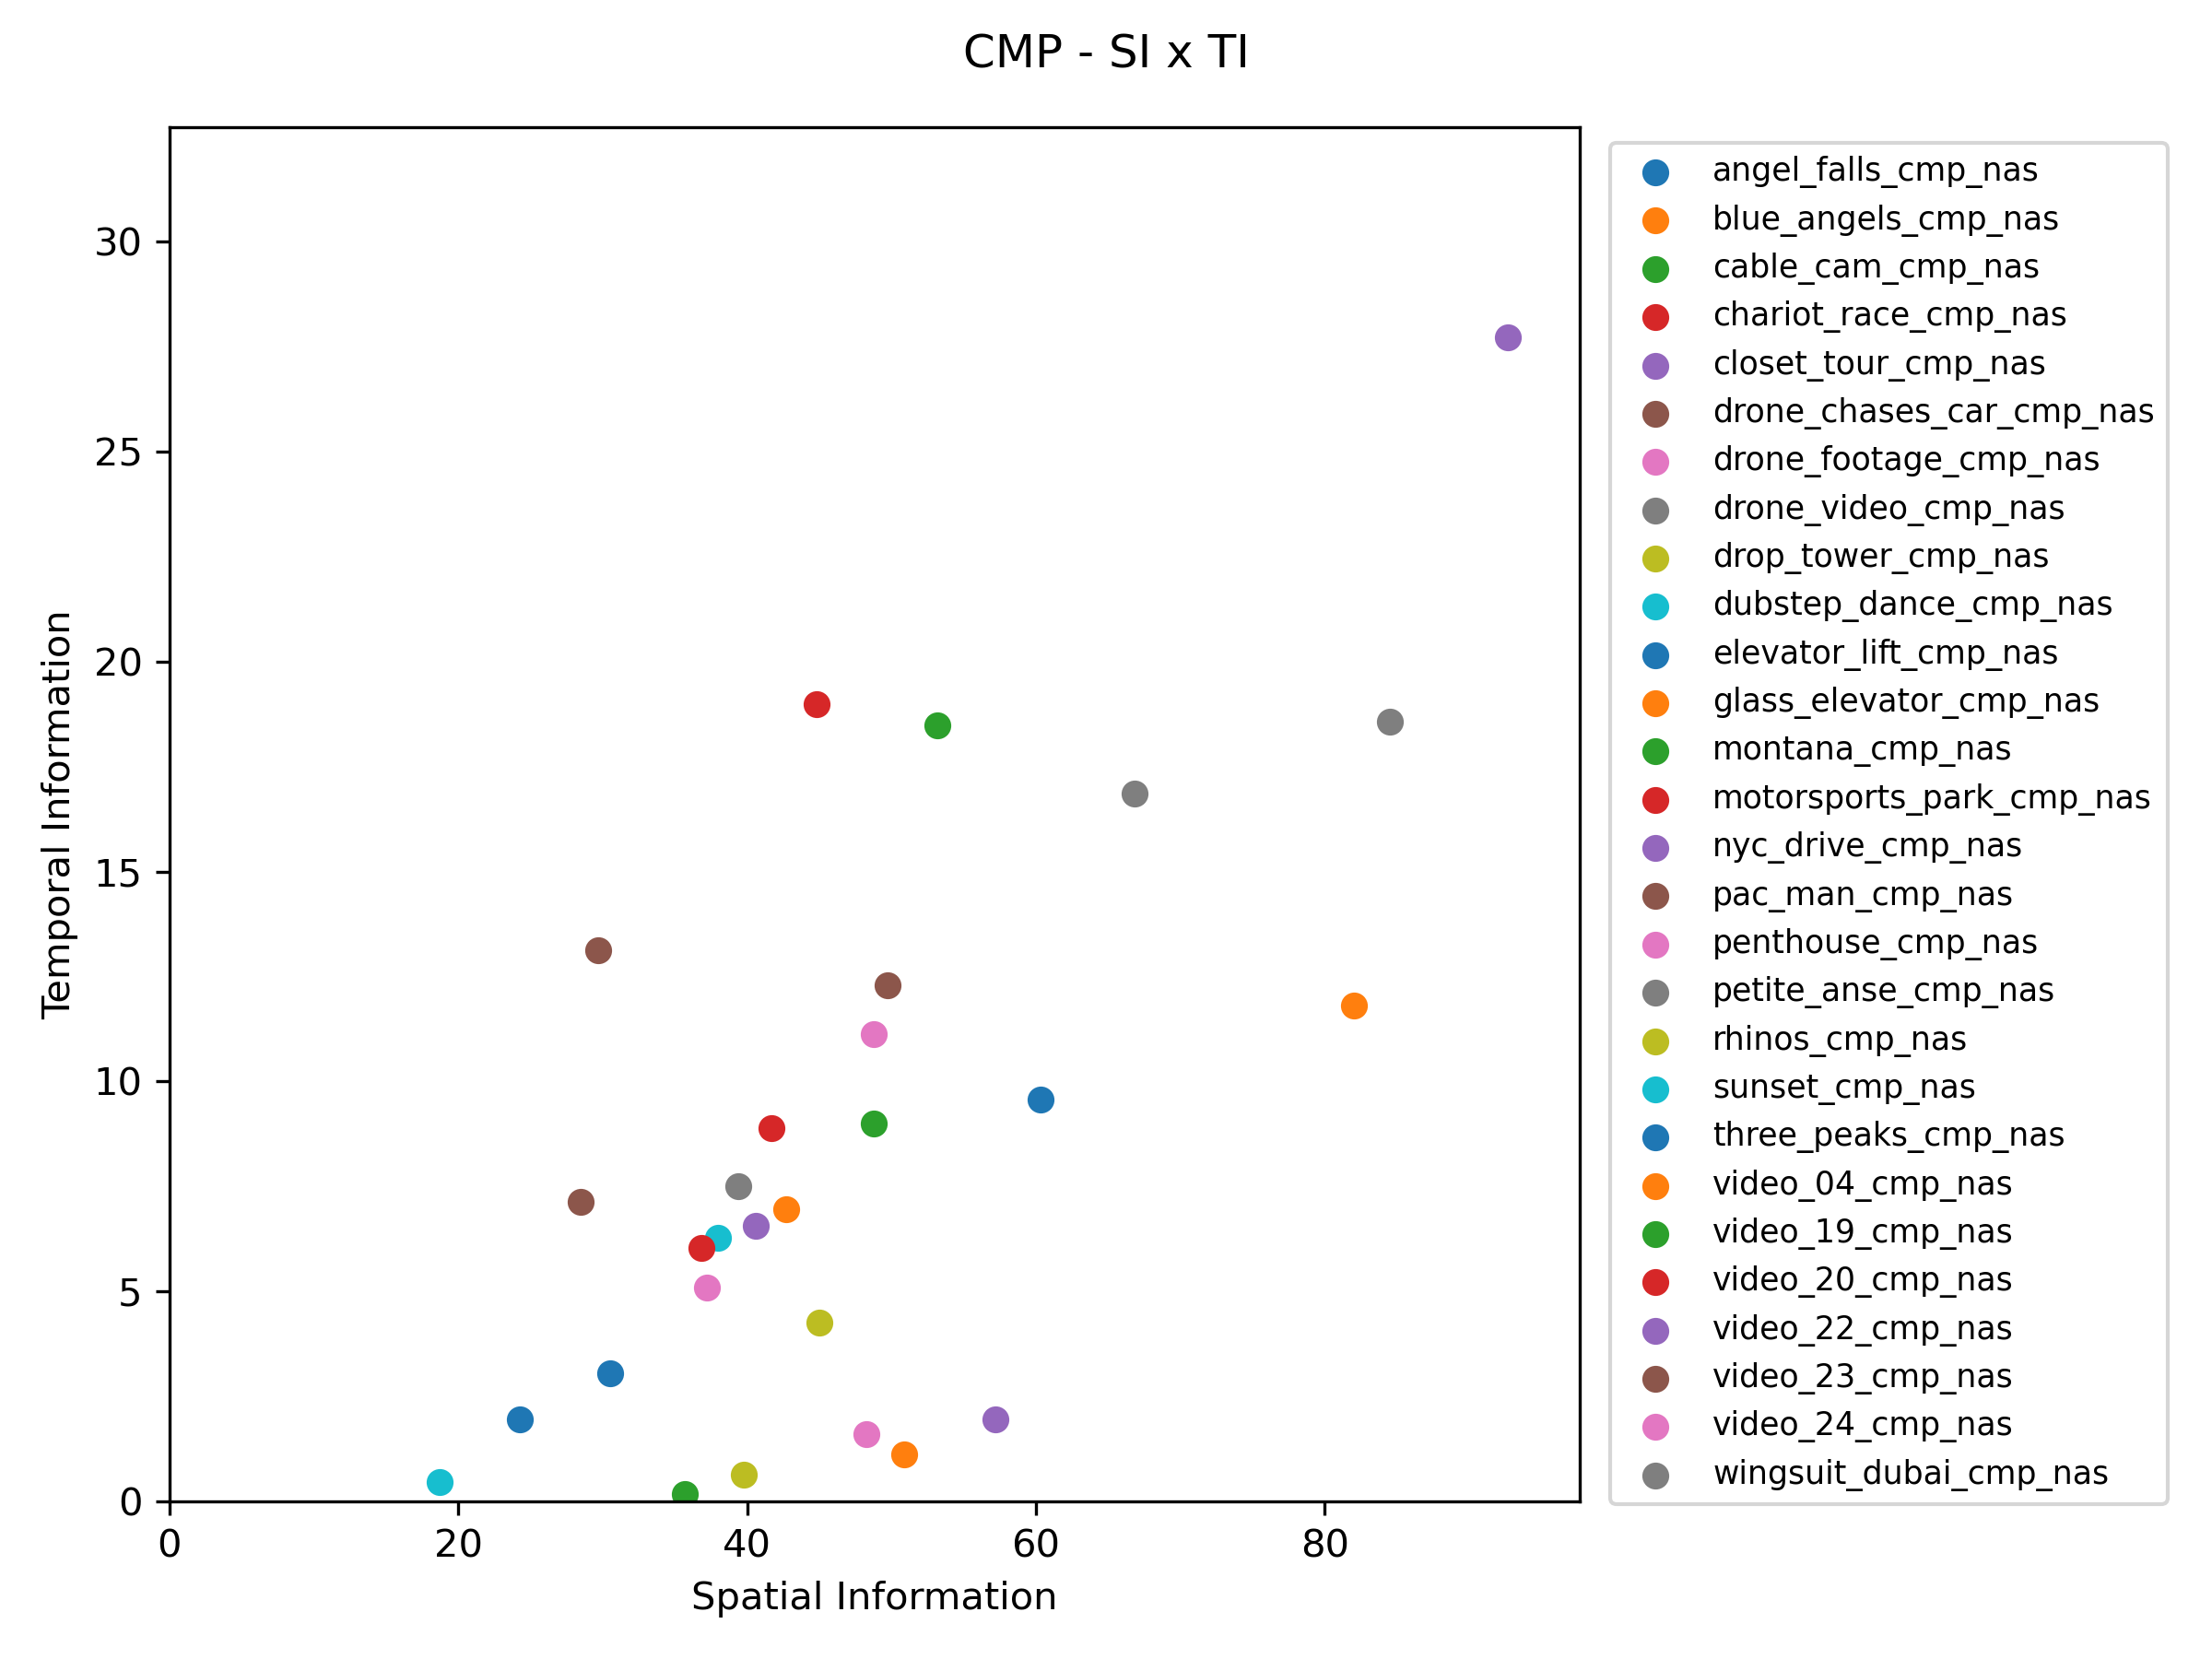
\includegraphics[width=0.45\linewidth]{fig/scatter_CMP.png}
        } % end subfigure
        \quad % dá um espaço entre as duas figuras.
        \subfigure[Projeção ERP. \label{fig:scatter_ERP}]{
                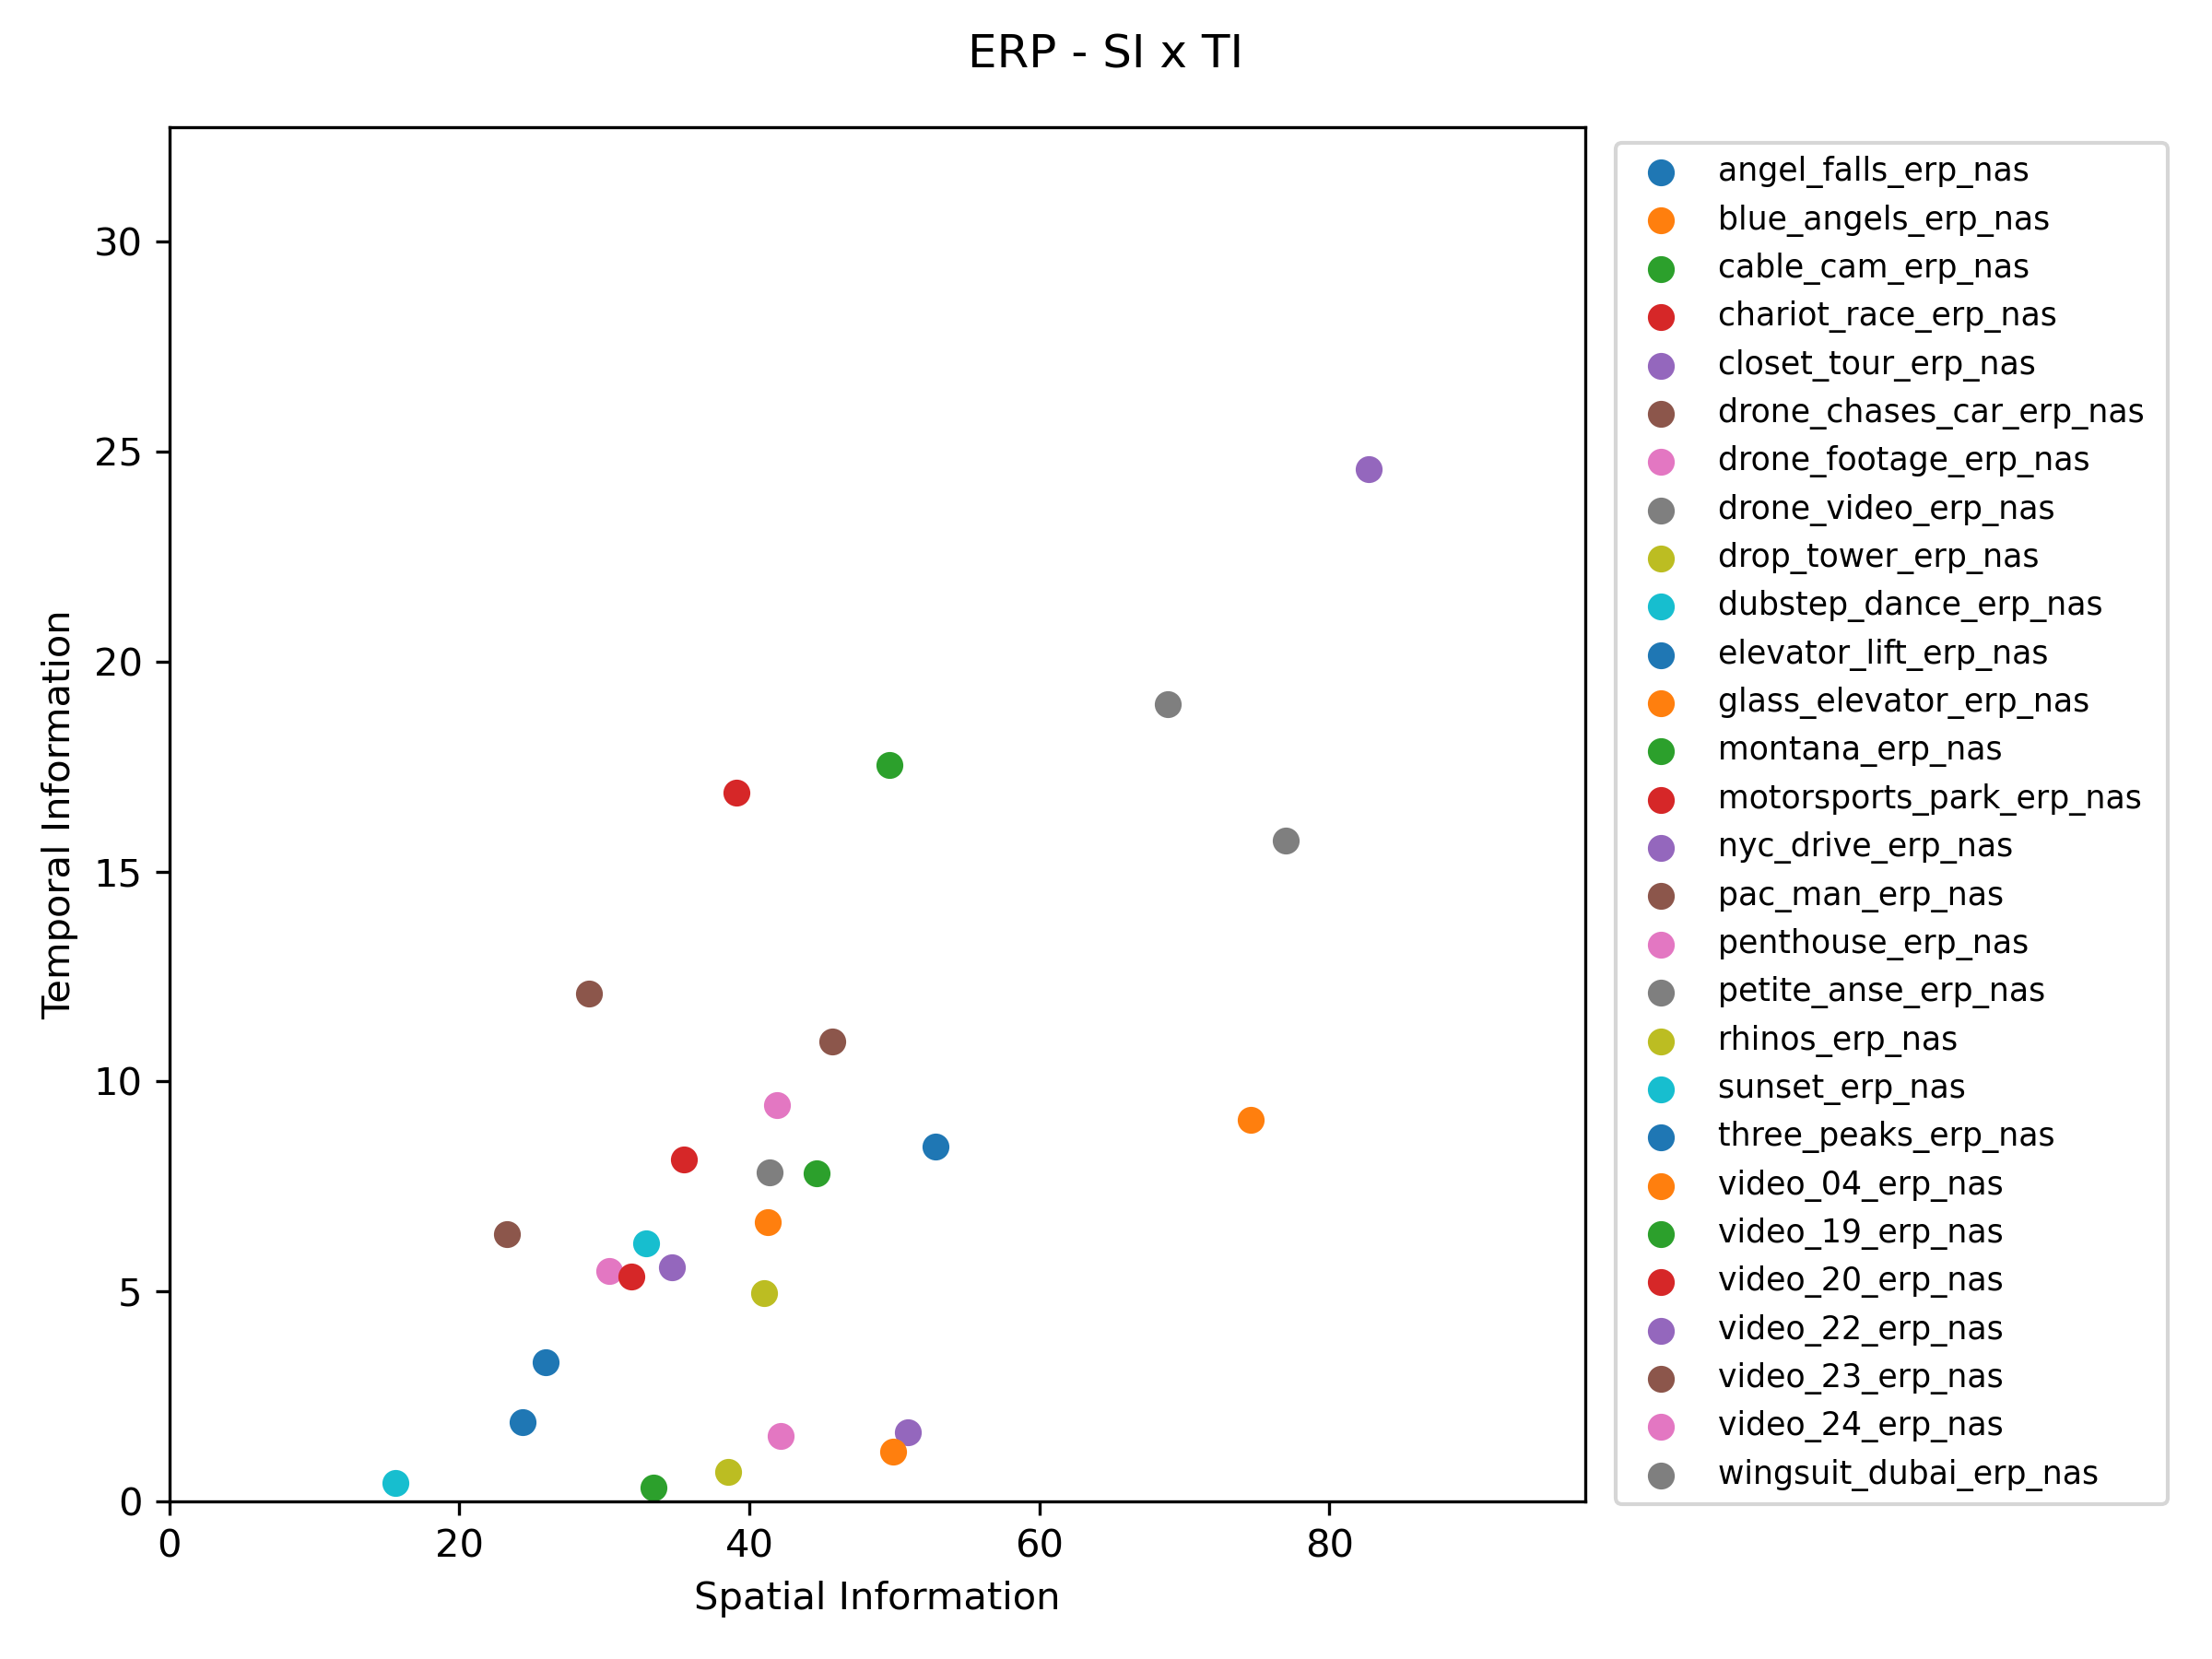
\includegraphics[width=0.45\linewidth]{fig/scatter_ERP.png}
        } % end subfigure
        \caption{Dispersão do SI e TI para as projeções avaliadas}
        \label{fig:scatter_si_ti}
\end{figure}

Para replicar uma condição comparável DASH-SRD, os ladrilho passaram pelo ladrilhamento antes da codificação, garantindo que cada ladrilho fosse espacialmente independente. Para cada vídeo, geramos quatro novas sequências de vídeo, cada uma com padrões de os ladrilhos conforme a tabela~\ref{tab:ladrilhamento_resolucoes}. Quanto maior o numero de ladrilhos, menor o numero de pixel em cada ladrilho, reduzindo o espaço de busca do compensador de movimento do codificador e reduzindo a eficiência da compressão. A projeção cúbica, tendo proporção menor tende a ser uma representação mais compacta, apresentando menor taxa de bits, porém com maior complexidade de compressão. Apesar de quanto menor os ladrilhos, menos pixels não visto são processador, este procedimento produz redução na eficiência do codificador. Além disso, quanto mais ladrilhos forem solicitados, serão necessárias múltiplas instâncias de um decodificador no cliente e mais complexo será o processo, pois para reproduzir um único quadro do ladrilho, todo o chunk precisa ser decodificado.


Subsequentemente, utilizamos o codificador HEVC x265 no FFmpeg\footnote{https://ffmpeg.org/} para padronizar e codificar cada ladrilho, empregando seis valores distintos do Fator de Taxa Constante (CRF) para controlar a qualidade/taxa de bits: 16, 22, 28, 34, 40 e 46. O valor de CRF mais baixo (mais alto) de 16 (46) corresponde à maior (menor) qualidade de vídeo. O valor padrão de 28 é recomendado pelo codificador por seu equilíbrio entre qualidade e taxa de compressão. Vale ressaltar que cada incremento de 3 no valor de CRF resulta em uma redução pela metade na taxa de bits; em nosso conjunto, a taxa de bits diminui quatro vezes para os valores de CRF especificados. Os parâmetros de codificação do vídeo estão detalhados na Tabela \ref{tab:parametros_qlt}. O GOP do vídeo foi fixado em 30 quadros, o parâmetro para detecção de cortes de cena foi desativado para que o GOP não varie dentro de um chunk e o parâmetro "--no-info" foi utilizado para omitir cerca de 200 bytes de informações sobre o codificador no cabeçalho mp4 e assim reduzir o overhead dos vídeos. Esta quantidade é relativamente significativa quando se trata de chunks muito pequenos com baixa complexidade de codificação e alta compressão. Além disso os vídeos foram processados com os parâmetros "-tune psnr" para comparação mais precisa das métricas de distorção, como MSE e PSNR. 

\begin{table}[htb]
        \centering
        \footnotesize
        \begin{tabular}{|l|c|}
                \hline
                \textbf{Resolução (Projeção)} & \makecell{$4320\times2160$ pixels (Cubemap), \\$3240\times2160$ pixels (Equirectangular)} \\ \hline
                \textbf{Taxa de Quadro} & 30 fps \\ \hline
                \textbf{GOP} & 30 quadros \\ \hline
                \textbf{Duração do Chunk} &  1 segundo \\ \hline
                \textbf{Qualidade (CRF)} & 0, 16, 22, 28, 34, 40 e 46 \\ \hline
                \textbf{Padrão de Ladrilho} & \makecell{$1\times 1$, $3 \times 2$, $6 \times 4$,  $9 \times 6$, $12\times 8$} \\ \hline
                \textbf{Codificador/Decodificador} & x265/FFmpeg 5.0-static \\ \hline
                \textbf{Configuração do x265} & keyint=30:min-keyint=30:open-gop=0:scenecut=0:info=0 \\ \hline
                \textbf{Sistema Operacional} & Ubuntu 22.04 \\ \hline
        \end{tabular}
        \caption{Parâmetros de codificação.}
        \label{tab:parametros_qlt}
\end{table}

Após a codificação, usando o programa GPAC\footnote{https://github.com/gpac/gpac/}, cada ladrilho passou por uma segmentação temporal em fragmentos de 1 segundo, equivalentes a um GOP (Grupo de Quadros) completo de 30 quadros. Essa escolha considera que a previsão de movimento da cabeça tende a ser eficaz dentro de janelas de previsão de aproximadamente 1-2 segundos~\cite{Qian2016}. Subsequentemente, esses fragmentos foram encapsulados em um arquivo MP4 para facilitar a decodificação individual, acarretando em um overhead de cerca de 100-1000 bytes para incluir um cabeçalho MP4 adicional de "box moov" por fragmento. Apesar do overhead, esta abordagem permite a decodificação independente de cada chunk por qualquer tocador de vídeo. Desta forma, cada ladrilho de cada vídeo em cada projeção, compreende 60 fragmentos decodificáveis em seis qualidades diferentes, resultando em um total de 3.648.960 \textit{chunks} para análise.

O processo de decodificação de vídeo ocorreu em um computador desktop i7-4770 de 3,4 GHz equipado com 16 GB de RAM, rodando Linux Ubuntu 22.04. O decodificador nativo do FFmpeg foi utilizado, empregando apenas uma thread para a decodificação. As medidas de tempo de decodificação coletadas apresentam precisão de 1 ms e são relativas ao tempo de usuário (\textit{user time}), o que representa o tempo da CPU, excluindo operações do kernel como chamadas de sistema, focando especificamente em tarefas de decodificação, como operações matriciais, por exemplo. Cada fragmento de um dado ladrilho passou por decodificação cinco vezes para produzir um tempo médio de decodificação. Devido a natureza multiprocesso e da hierarquia de memória, foi possível observar uma variação do tempo de decodificação de até 93,75\%. Além disso, medimos a taxa de bits de cada \textit{chunk} simplesmente multiplicando o tamanho do arquivo por oito, já que cada \textit{chunk} possui exatamente 1 segundo.

A seguir, para cada quadro de cada chunk, métricas objetivas de qualidade, incluindo SSIM, MSE, WS-MSE e S-MSE, serão calculadas comparando os quadros decodificados os vídeos codificados com CRF 0. As métricas são armazenadas em um JSON em uma estrutura de árvores, em que cada nível representa respectivamente a projeção, nome do video, padrão de ladrilhamento, crf, ladrilho e chunk. No caso do tempo de decodificação, foi armazenado um valor para cada decodificação.

Para a análise das distribuições estatística dos chunks codificados, empregamos a biblioteca Python SciPy. Por padrão, a SciPy utiliza do método de Estimação por Máxima Verossimilhança para determinar os parâmetros da distribuições de probabilidade de densidade (PDF). As distribuições analisadas são: Burr Tipo XII , Birnbaum-Saunders, Gamma, Inversa Gaussiana, Rayleigh, Log Normal, Generalized Pareto, Pareto, Half-Normal, e Exponencial\footnote{https://docs.scipy.org/doc/scipy/reference/stats.html}. Como ferramenta auxiliar foi utilizado o pacote Fitter para testar todas as distribuições\footnote{https://fitter.readthedocs.io/}. Além das distribuições foi analisada a correlação entre as métricas e para a avaliação dos erros, foi utiliza a raiz do erro quadrático médio (RMSE). Nos resultados produzidos pela Scipy, os valores são normalizados e os parâmetros de deslocamento ({\it loc}) e escala ({\it scale}) devem ser aplicados à distribuição normalizada para obter a ajustada, conforme a equação~\ref{eq:shift_scale}.

\begin{equation}
        \label{eq:shift_scale}
        \text{fitted\_pdf}(x) = \left( \frac{1}{scale} \right) \text{normalized\_pdf}\left(\frac{x-loc}{scale}\right).
\end{equation}


\section{Caracterização dos elementos do cliente}

% kd o diagrama?
Para a caracterização do que o usuário experimenta, a posição da cabeça do usuário é utilizada para identificar as ladrilhos necessárias para a reconstrução da viewport. Foi desenvolvido uma bibliteca para conversão de coordenadas na esfera e um mecanismo para seleção de ladrilhos com base na posição da cabeça do usuário. Este mecanismo foi implementado em Python, e, quando fornecido o padrão de ladrilhamento, dimensões da projeção e posição da viewport, ele retorna uma lista de ladrilhos que estão visíveis na viewport. Existem vários métodos para selecionar e priorizar ladrilhos~\cite{Nguyen2020}. Porém, neste trabalho, focamos em considerar apenas os ladrilhos visíveis, essenciais para a construção da viewport, conforme ilustrado na Figura~\ref{fig:tilesSelection}. Este mecanismo foi aplicado com um banco de dados de posição da cabeça do usuário para calcular uma lista de ladrilhos que aparecem na viewport durante a reprodução.

\begin{figure}[htb]
        \centering
        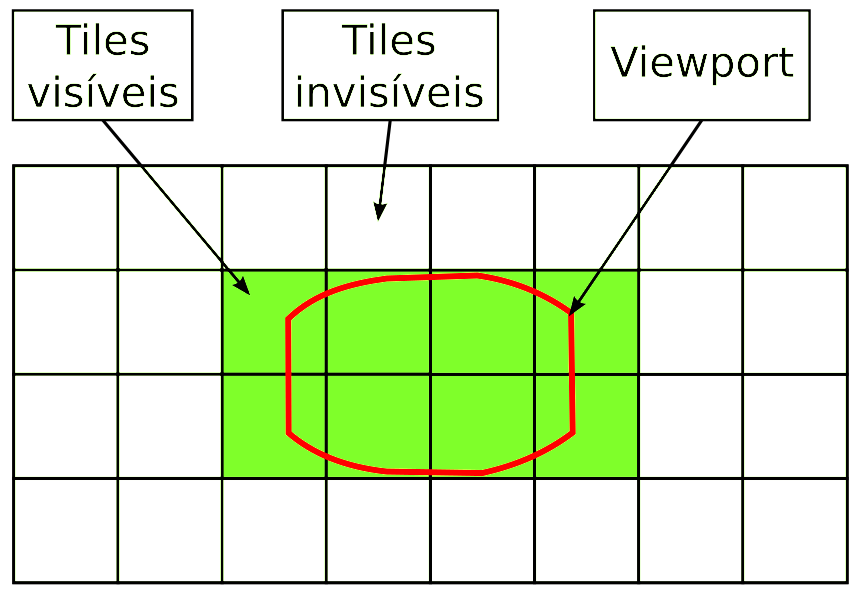
\includegraphics[width=0.6\linewidth]{fig/tiles selection simples.png}
        \caption{Mecanismo para seleção de ladrilhos.}
        \label{fig:tilesSelection}
\end{figure}

O banco de dados de movimentos da cabeça foi gerado por Nasrabadi \cite{Nasrabadi2019}. Este banco de dados compilou a posição central do viewport na esfera para 60 voluntários (30 voluntários por vídeo), representados em quatérnions e em vetores cartesianos a uma taxa variável. Utilizando marcas de tempo foi feita a interpolação para que todas as amostras estejam à taxa de 30 Hz. A figura \ref{fig:datasetSpeedmap}, extraída do trabalho de Nasrabadi, fornece um mapa da velocidade angular média para todos os usuários em cada vídeo. Como observado pelo autor, a velocidade angular média dos vídeos depende do usuário, o que significa que um usuário com velocidade alta em um vídeo tende a exibir velocidade alta em todos os vídeos. 

\begin{figure}
        \centering
        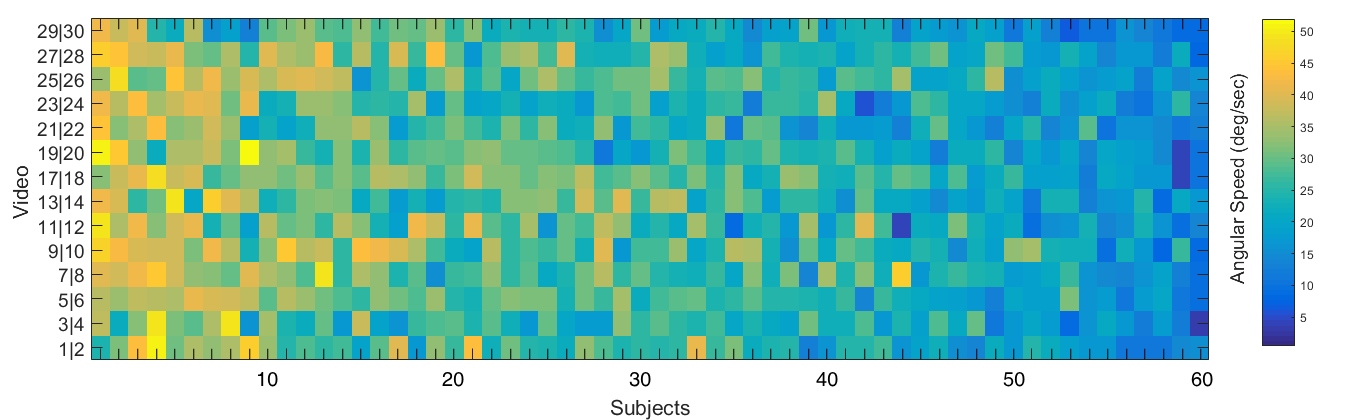
\includegraphics[width=0.8\linewidth]{fig/datasetSpeedmap.png}
        \caption{Mapa da velocidade angular média de todos os voluntários para todos os grupos de vídeo. Extraído de  \cite{Nasrabadi2019}}
        \label{fig:datasetSpeedmap}
\end{figure}

A seguir, considerando os ladrilhos selecionados na etapa anterior, são reconstruídos a projeção e geradas viewports tanto de vídeos não compactados (CRF 0) quanto de vídeos codificados com qualidade variável para uma mesma região, com base nas regiões que os indivíduos visualizaram anteriormente. nas regiões da projeção que o ladrilho não foi selecionado é preenchido com zero. A criação da viewport é realizada utilizando a projeção Gnomônica (chamada também de projeção retilinear) restrita pelo campo de visão (FOV) do dispositivo. Nossa janela de visualização é configurada com um FOV horizontal e vertical de 100°x90°, um valor aproximado daqueles adotados pela linha Oculus Quest~\footnote{https://risa2000.github.io/hmdgdb/}. A seguir, será calculado o PSNR entre o quadro da viewport criado com ladrilhos compactados e o quadro da viewport criado com ladrilhos não compactados (com CRF 0).


\section{Cenários avaliados}

Após a coleta dos dados, o comportamento da qualidade será analisado sob duas perspectivas: uma do ponto de vista de um sistema ABR que considera a correlação da qualidade com a taxa de transmissão do vídeo e outra do ponto de vista do usuário que visualiza o vídeo utilizando óculos de realidade virtual. 

\subsection{Estatísticas dos ladrilhos por ladrilhamento}

A tabela~\ref{tab:stats} fornece os valores de média e desvio padrão para o tempo de decodificação e a taxa de bits dos \textit{chunk} para vários padrões de ladrilho. Conforme previsto, a redução no tamanho do ladrilho (correspondendo a um aumento no ladrilhamento do vídeo) menor a taxa de bits e o tempo de decodificação por ladrilho. O desvio padrão da taxa de bits apresenta um valor superior à média, pois esta média inclui todas as qualidades, o que resulta em uma variação de aproximadamente 20 vezes na taxa de bits. Além disso, a projeção cúbica possui uma taxa de bits média aproximadamente 8\% menor do que a projeção equirretangular. Isto se deve a sua representação ser mais compacta e exigir menos pixels. Esta diferença também se reflete no tempo de decodificação dos ladrilhos que serão decodificados mais rapidamente. 
A tabela também revela que as métricas de qualidade sofrem um sutil aumento com o aumento do ladrilhamento enquanto seu desvio padrão cresce de forma mais agressiva. Esta variação ocorre porque o codificador, configurado com o parâmetro CRF, ajusta a quantização afim de manter a qualidade uniforme\footnote{https://x265.readthedocs.io/en/master/cli.html} e uma vez que o ladrilhamento isola regiões da projeção que possuem atividade espacial e temporal diferente, o codificação aplicará a quantização de forma diferente, aumentando o desvio padrão e deslocando a média. % A métrica S-MSE está errada, parece que eu calculei a média em cima dos pixels da projeção e não dos pixels do ladrilho.
Já a métrica SSIM não apresenta diferença significativa entre os ladrilhamentos, apesar de seu desvio padrão aumentar com a redução dos ladrilhos. Quando comparamos as métricas de qualidade para as diferentes projeções, vemos que a projeção equirretangular apresenta m

\begin{longtable}{|c|c|c|c|c|c|}
        \caption{Valores de média e desvio padrão das métricas analisadas de acordo com o ladrilhamento, abrangendo todas qualidades.} \label{tab:stats} \\
        
        \hline
        \multirow{2}{*}{\textbf{Métrica}} &  \multirow{2}{*}{\textbf{Ladrilhamento}} & \multicolumn{2}{c|}{\textbf{CMP}} & \multicolumn{2}{c|}{\textbf{ERP}} \\
        \cline{3-6}
        &   & \textbf{Média} & \textbf{Desvio Padrão} & \textbf{Média} & \textbf{Desvio Padrão} \\
        \hline
        \endfirsthead
        
        \multicolumn{6}{c}%
        {{\bfseries \tablename\ \thetable{} -- Continuação da página anterior}} \\
        \hline
        \endhead
        
        \hline \multicolumn{6}{|r|}{{Continua na próxima página}} \\ \hline
        \endfoot
        
        \hline
        \endlastfoot
        
        \multirow{5}{*}{Taxa}  & 1x1  & 6.050.720 & 10.352.018 & 6.591.315 & 11.176.695 \\ \cline{2-6}
        & 3x2  & 1.030.891 & 2.012.731  & 1.130.073 & 2.281.468 \\ \cline{2-6}
        & 6x4  & 277.689   & 589.369    & 301.493   & 661.050  \\  \cline{2-6}
        & 9x6  & 133.972   & 273.547    & 144.640   & 318.278  \\  \cline{2-6}
        & 12x8 & 84.727    & 163.725    & 90.798    & 188.049  \\   \hline
        \multirow{5}{*}{Tempo} & 1x1  & 0,629     & 0,278      & 0,757     & 0,311     \\  \cline{2-6}
        & 3x2  & 0,098     & 0,053      & 0,122     & 0,062    \\  \cline{2-6}
        & 6x4  & 0,022     & 0,015      & 0,026     & 0,017    \\  \cline{2-6}
        & 9x6  & 0,011     & 0,007      & 0,012     & 0,008    \\  \cline{2-6}
        & 12x8 & 0,006     & 0,004      & 0,008     & 0,005    \\  \hline 
        % \pagebreak\hline
        \multirow{5}{*}{MSE}   & 1x1  & 21,472    & 33,788     & 17,782    & 28,024    \\  \cline{2-6}          
        & 3x2  & 21,603    & 39,575     & 18,155    & 34,290   \\  \cline{2-6}
        & 6x4  & 21,923    & 45,121     & 18,409    & 39,623   \\  \cline{2-6}
        & 9x6  & 22,523    & 48,846     & 18,853    & 43,182   \\  \cline{2-6}
        & 12x8 & 22,613    & 50,499     & 19,034    & 45,037   \\  \hline 
        \multirow{5}{*}{SSIM}  & 1x1  & 0,951     & 0,050      & 0,957     & 0,043     \\  \cline{2-6}
        & 3x2  & 0,951     & 0,060      & 0,957     & 0,055    \\  \cline{2-6}
        & 6x4  & 0,951     & 0,068      & 0,957     & 0,061    \\  \cline{2-6}
        & 9x6  & 0,951     & 0,071      & 0,957     & 0,064    \\  \cline{2-6}
        & 12x8 & 0,951     & 0,073      & 0,957     & 0,067    \\  \hline 
        \multirow{5}{*}{WS-MSE}& 1x1  & 21,784    & 33,965     & 20,473    & 33,051   \\  \cline{2-6}
        & 3x2  & 21,968    & 40,410     & 20,880    & 39,442   \\  \cline{2-6}
        & 6x4  & 22,420    & 45,615     & 19,578    & 42,162   \\  \cline{2-6}           
        & 9x6  & 22,738    & 49,216     & 19,401    & 44,243   \\  \cline{2-6}                
        & 12x8 & 22,758    & 50,740     & 19,343    & 45,660   \\  \hline 
        \multirow{5}{*}{S-MSE}  & 1x1  & 21,779    & 34,009     & 20,461    & 33,072   \\  \cline{2-6}
        & 3x2  & 3,661     & 6,749      & 3,477     & 6,572    \\  \cline{2-6}
        & 6x4  & 0,935     & 1,904      & 0,883     & 2,084    \\  \cline{2-6}
        & 9x6  & 0,427     & 0,963      & 0,401     & 1,014    \\  \cline{2-6}
        & 12x8 & 0,241     & 0,568      & 0,228     & 0,597 
\end{longtable}

A figura~\ref{Fig:boxplottiling} mostra o boxpplot para cada métrica. Cada caixa representa o segundo e o terceiro quartil e a linha interna representa a mediana. Os traços acima e abaixo da caixa representam os valores máximos e mínimos. Apesar do desvio padrão ser alto, a maior parte dos valores estão concentrados em torno da mediana, indicando que, apesar da alta variação nestas métricas, apenas em poucos casos ocorrerão desvios.

\begin{figure}[htb]
         \centering         

           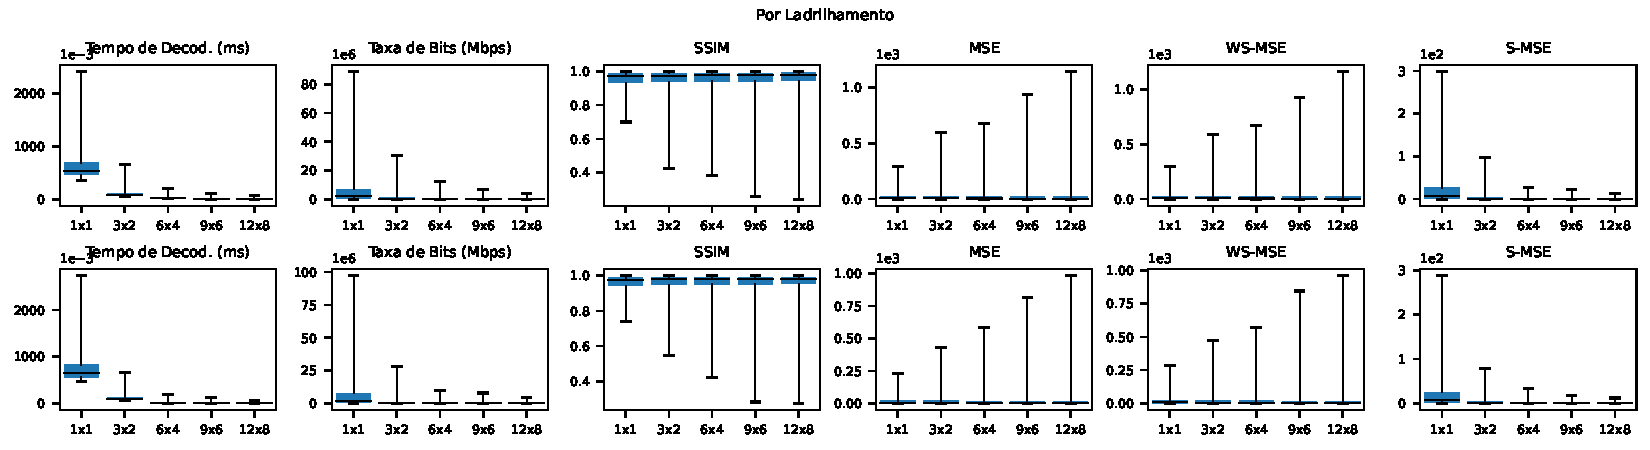
\includegraphics[width=0.9\columnwidth]{fig/ByPattern/boxplot_pattern.pdf}
           \caption{Boxplot do tempo de decodificação, taxa de bits e erro organizado por ladrilhamento.}
           \label{Fig:boxplottiling}
\end{figure}


A Figura ~\ref{Figura:histograma-fmt} descreve, para cada padrão de ladrilho, as três melhores funções de densidade de probabilidade ajustadas à distribuição empírica do tempo de decodificação do ladrilho. A partir dos resultados, a distribuição Log-Normal está entre as três distribuições mais bem ajustadas em 100\% dos padrões, enquanto as distribuições Gaussiana Inversa e Birnbaum-Saunders aparecem em 87,5\% e 75\% dos casos, respectivamente.


%%%%%%%%%%%
%% Statistic By Quality
%%%%%%%%%%%
\subsection{Estatísticas por nível de qualidade e ladrilhamento}

%Corrigir estes valores
A Figura ~\ref{Figura:bar-fmt-qlt} ilustra o tempo médio de decodificação do ladrilho e a taxa de bits média por nível de qualidade para cada padrão de ladrilho. A redução na taxa de bits correspondente a uma diminuição na qualidade do vídeo é acompanhada por uma diminuição semelhante, embora menos pronunciada, no tempo de decodificação dos blocos. Por exemplo, no cenário $6 \times 4$, onde a taxa de bits diminui em 97,5\% (de 1,91 Mbps para 47,6 Kbps) em uma faixa CRF de 16 a 46, o tempo de decodificação do bloco diminui apenas 63,1\% (de 0,067 a 0,025 segundos) para a mesma faixa CRF.

Analisando os resultados, fica evidente que as três distribuições mais bem ajustadas variam de acordo com o padrão de ladrilho. As frequências com que aparecem entre os três primeiros são as seguintes: Birnbaum-Saunders (79,2\%), Gaussiana Inversa (72,9\%), Log-Normal (70,8\%), Burr Tipo XII (41,7\%), Gama (8,33\%), Pareto Generalizado (8,3\%), Half Normal (6,3\%), Exponencial (3,08\%) e Rayleigh (2,1\%).

% \begin{figure*}[hbt]
        % \centering
        %   \includegraphics[width=2\columnwidth]{fig/bar_fmt-quality_30bins_crf.png}
        %   \caption{Tempo médio de decodificação para blocos (representado por barras azuis) e taxa de bits média (representada por linhas vermelhas) categorizados por padrão de ladrilho e nível de qualidade do ladrilho.}
        %   \label{Figure:bar-fmt-qlt}
        % \end{figure*}

Tabela~\ref{tab:corr_list} fornece os resultados da correlação entre o tempo de decodificação do bloco e a taxa de bits média em todos os casos. Notavelmente, para um determinado padrão de ladrilhos, a correlação tende a aumentar com níveis de qualidade mais elevados. Por outro lado, para um determinado valor de CRF, a correlação diminui à medida que o número de blocos por quadro aumenta.

Como ilustração, considerando o padrão de ladrilhos de $6 \times 3$, a correlação é de aproximadamente 0,728 para CRF = 28. É digno de nota que esse padrão de ladrilhos específico demonstrou alcançar economias substanciais de largura de banda em pesquisas anteriores~\cite{Graf2017}.

\begin{table}[htb]
        \footnotesize
        \caption{Correlação entre o tempo de decodificação do bloco e a taxa de bits do bloco.}
        \label{tab:corr_list}
        \begin{center}
                \begin{tabular}{|c|c|c|c|c|c|c|}
                        \hline
                        \multirow{2}{*}{\textbf{Padrão}} & \multicolumn{6}{c|}{\bf Qualidade (CRF)} \\
                        \cline{2-7}
                        & \textbf{16} & \textbf{22} & \textbf{28} & \textbf{34} & \textbf{40} & \textbf{46} \\
                        \hline
                        $1\times 1$ & 0.893 & 0.839 & 0.803 & 0.786 & 0.704 & 0.554 \\
                        \hline
                        $3\times 2$ & 0.857 & 0.781 & 0.735 & 0.684 & 0.610 & 0.479 \\
                        \hline
                        $4\times 3$ & 0.846 & 0.782 & 0.744 & 0.674 & 0.584 & 0.497 \\
                        \hline
                        $6\times 3$ & 0.848 & 0.788 & 0.734 & 0.683 & 0.581 & 0.471 \\
                        \hline
                        $6\times 4$ & 0.843 & 0.789 & 0.728 & 0.673 & 0.566 & 0.451 \\
                        \hline
                        $6\times 5$ & 0.827 & 0.761 & 0.703 & 0.636 & 0.537 & 0.424 \\
                        \hline
                        $6\times 6$ & 0.814 & 0.748 & 0.687 & 0.617 & 0.520 & 0.403 \\
                        \hline
                        $7\times 6$ & 0.808 & 0.743 & 0.688 & 0.605 & 0.505 & 0.398 \\
                        \hline
                \end{tabular}
        \end{center}
\end{table}

%%%%%%%%%%%
%% Full-Frame Statistic
%%%%%%%%%%%
\subsection{Estatísticas dos \textit{Chunks} para o envio de todos o ladrilhos}

Agora, nosso foco muda para o tempo necessário para decodificar sequencialmente todos os ladrilhos de um intervalo de tempo, considerando todos os vídeos e níveis de qualidade coletivamente. Desta forma poderemos simular o pior caso, onde o usuário terá que solicitar e processar toda a esfera. A Figura~\ref{Figura:bar-fmt} ilustra o tempo médio de decodificação do pedaço e a taxa de bits média para cada padrão de ladrilho, com barras de erro indicando o desvio padrão.

Como previsto, a taxa de bits apresenta um aumento correspondente ao aumento no número de blocos por quadro. Este resultado é atribuído ao fato de que a segmentação de blocos restringe o espaço de busca para a previsão de movimento do codificador. Inesperadamente, o tempo médio de decodificação do bloco se beneficia da segmentação lado a lado, com valores médios geralmente menores que aqueles observados para o caso $1 \times 1$. Observa-se que o tempo médio de decodificação diminui à medida que o número de ladrilhos por quadro aumenta, atingindo um mínimo no ladrilhamento $6 \times 3$. Esse mínimo é aproximadamente 10,8\% menor que o padrão $1 \times 1$, e essa melhoria é alcançada com apenas um aumento de 6,26\% na taxa de bits. Além deste ponto, os valores do tempo de decodificação começam a subir novamente. As razões específicas por trás deste comportamento merecem uma investigação mais aprofundada, pois a complexidade do vídeo codificado reduz a medida que os ladrilhos diminuem de tamanho, tornando mais rápido a decodificação do conjunto, porém o número de bits aumenta, o que aumentaria o tempo de decodificação. Contudo, a exploração desta ocorrência está além do escopo deste trabalho.

% \begin{figure}[htb]
        %     \centering
        %     \includegraphics[width=0.8\columnwidth]{fig/bar_fmt-dectime_x_time_ts.png}
        %     \caption{Tempo de decodificação de pedaços e taxa de bits média por padrão de ladrilho.}
        %     \label{Figure:bar-fmt}
        % \end{figure}

Nossas medições revelam uma correlação significativa entre o tempo médio de decodificação do chunk e sua taxa de bits média em todos os padrões de ladrilhos. O coeficiente de correlação medido ultrapassa 0,96 em todos os casos. A Figura~\ref{Figura:hist-somafmt} ilustra as três distribuições de probabilidade com menor erro para os dados coletados em cada padrão de ladrilho.

Notavelmente, as distribuições Gaussiana Inversa e Birnbaum-Saunders estão consistentemente classificadas entre as três primeiras em 100\% dos padrões, enquanto a distribuição Log-Normal aparece entre as três primeiras em 87,5\% dos padrões. A distribuição Burr Tipo XVII surge como uma candidata potencial para o caso $1 \times 1$. Infelizmente, os valores específicos dos parâmetros de distribuição para este caso não são apresentados devido a limitações de espaço.

% \begin{figure*}[htb]
        %         \centering
        %         \includegraphics[width=2\columnwidth]{fig/hist_60bins_fmt_somatiles_crf.png}
        %         \caption{O histograma de densidade do tempo de decodificação para todos os padrões de blocos e as três melhores distribuições com o RMSE menor, para o vídeo em blocos completo.}
        %         \label{Figure:hist-somafmt}
        % \end{figure*}


\subsection{Ladrilhos vistos (por viewport)}

No primeiro cenário, para cada chunk haverá um conjunto de ladrilhos que aparecem no viewport. Ao longo da duração do chunk o usuário poderá mover a cabeça e o conjunto de ladrilhos muda. Estes novos ladrilhos precisam já ter sido decodificados completamente para poderem ser exibidos. Desta forma é preciso considerar a trajetória do movimento de cabeça para se requisitar os ladrilhos. Sendo A o conjunto dos ladrilhos que são vistos pelo viewport no quadro f, os ladrilhos vistos $lv$ durante a duração de um chunk será dada pela equação~\ref{eq:tiles_seen}.

\begin{equation}
        lv=\bigcup^{30}_{f=1} A_f \\    
        \label{eq:tiles_seen}
\end{equation}

A taxa de bits de $lv$ será igual a soma da taxa de todos os ladrilhos de $lv$. Para o tempo de decodificação de $lv$, podemos ter duas abordagens. Decodificação em série: os ladrilhos de $lv$ são decodificados em série e o tempo total de decodificação de todos será igual a soma do tempo de todos os ladrilhos de $lv$. A segunda abordagem é a decodificação em paralelo: Neste caso o tempo de decodificação de $lv$ é definido pelo maior tempo de todos os ladrilhos de $lv$. Já a qualidade, devemos considerar a média do MSE, SSIM, S-MSE e WS-MSE de todos os ladrilhos em $lv$. Por fim, uma seção de vídeo $sv$ consiste de uma sequencia de $lv$ com tamanho igual ao numero de chunks de um vídeo. Em $sv$ temos todos os ladrilhos que foram vistos ao longo do vídeo separados em blocos de 1 segundo. Cada ladrilho tem associado sua posição espacial e temporal, indicada por um índice na lista de ladrilhos e pelo número do chunk que foi visto ao longo da reprodução. Como temos 30 usuários por vídeo, 28 vídeos, dois tipos de projeção e cinco tipos de ladrilhamento, teremos ao todo 8400 seções que podem ser reproduzidas considerando seis qualidades. Entre as métricas avaliadas, estão o número de ladrilhos utilizados pelo viewport ao longo da reprodução, taxa de bits, tempo de decodificação e qualidade do viewport e dos ladrilhos na projeção. Essa análise também pode ser estendida para diversas técnicas de seleção de ladrilho.


\chapter{Conclusão e Trabalhos Futuros}\label{Cap:Conclusion}

Este trabalho apresentou uma modelagem de transmissão de streaming de vídeo em 360 graus com ladrilhos que consideravam diferentes padrões de ladrilhamento em uma ampla faixa de níveis de qualidade de vídeo (isto é, taxas de bits) e propriedades SI/TI. A partir dos resultados, as distribuições Log-Normal, Gaussiana Inversa e Birnbaum-Saunders ajustaram-se melhor aos dados experimentais na maioria dos casos. Tais distribuições são muito flexíveis e interessantes para fins de modelagem matemática (por exemplo, aplicação a modelos de filas). O tempo de decodificação do ladrilho está fortemente correlacionado com a taxa de bits do ladrilhos somente se a qualidade do vídeo for alta, e o grau de correlação diminui se o número de ladrilhos por quadro aumentar (ou seja, alta segmentação do bloco). O padrão de ladrilho $6 \times 3$ proporcionou o melhor equilíbrio entre o tempo de decodificação e a taxa de bits média, ao mesmo tempo que apresentou boas propriedades de correlação entre ambas as métricas se altos níveis de qualidade forem usados. Tal informação pode possivelmente ser usada por algoritmos ABR baseados em DASH para inferir o tempo de decodificação dos ladrilhos.

Como trabalho futuro planejamos projetar um algoritmo de adaptação de qualidade utilizando as métricas de desempenho analisadas e então avaliá-lo em um ambiente virtual de simulação de rede usando o simulador NS-3\footnote{https://www.nsnam.org/} conectado a servidores locais reais rodando em containers Docker. Considerando o registro de movimento de cabeça e que todos os segmentos acessados pelo cliente serão sempre os mesmos para cada usuário, será possível avaliar diferentes tipos de algoritmos sob diferentes infraestruturas sob as mesmas condições de usuário. Então, usando o modelo de qualidade desenvolvido neste trabalho será possível avaliar de forma objetiva a capacidade dos algoritmos se adaptarem às condições de rede em um ambiente bem controlado, como o mostra a figura~\ref{fig:modelo_simulação}.

\begin{figure}[htb]
        \centering
        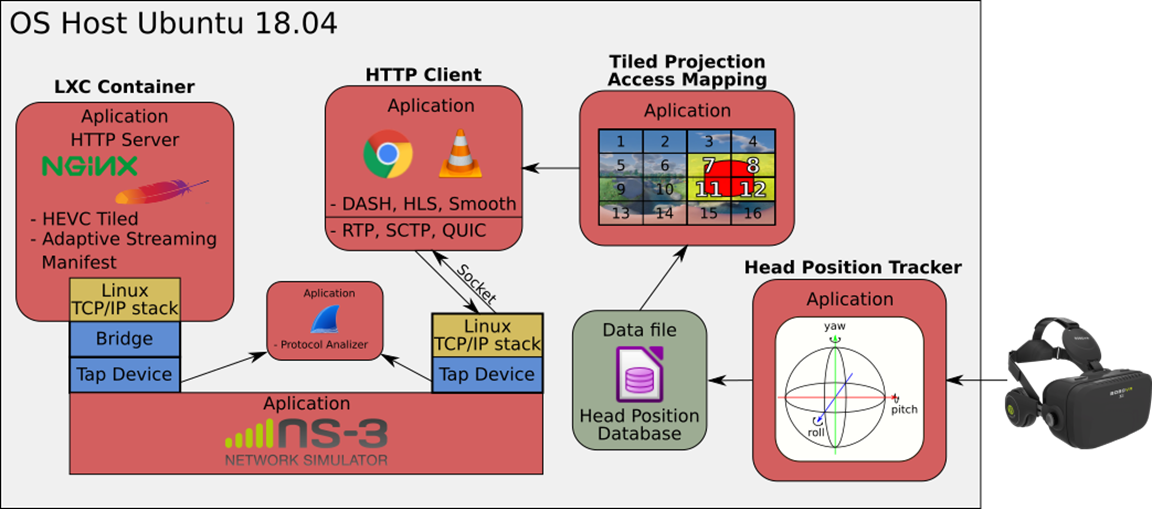
\includegraphics[width=0.8\linewidth]{fig/modelo_simulação.png}
        \caption{Modelo de simulação que será usado para avaliação}
        \label{fig:modelo_simulação}
\end{figure}


\section{Trabalhos futuros}

\section{Cronograma}


